\section{Overlap Studies}
\label{ch:OverlapStudies}

\begin{frame}{Do Bunches Collide Maximally Overlapped?}
\begin{figure}
\begin{center}
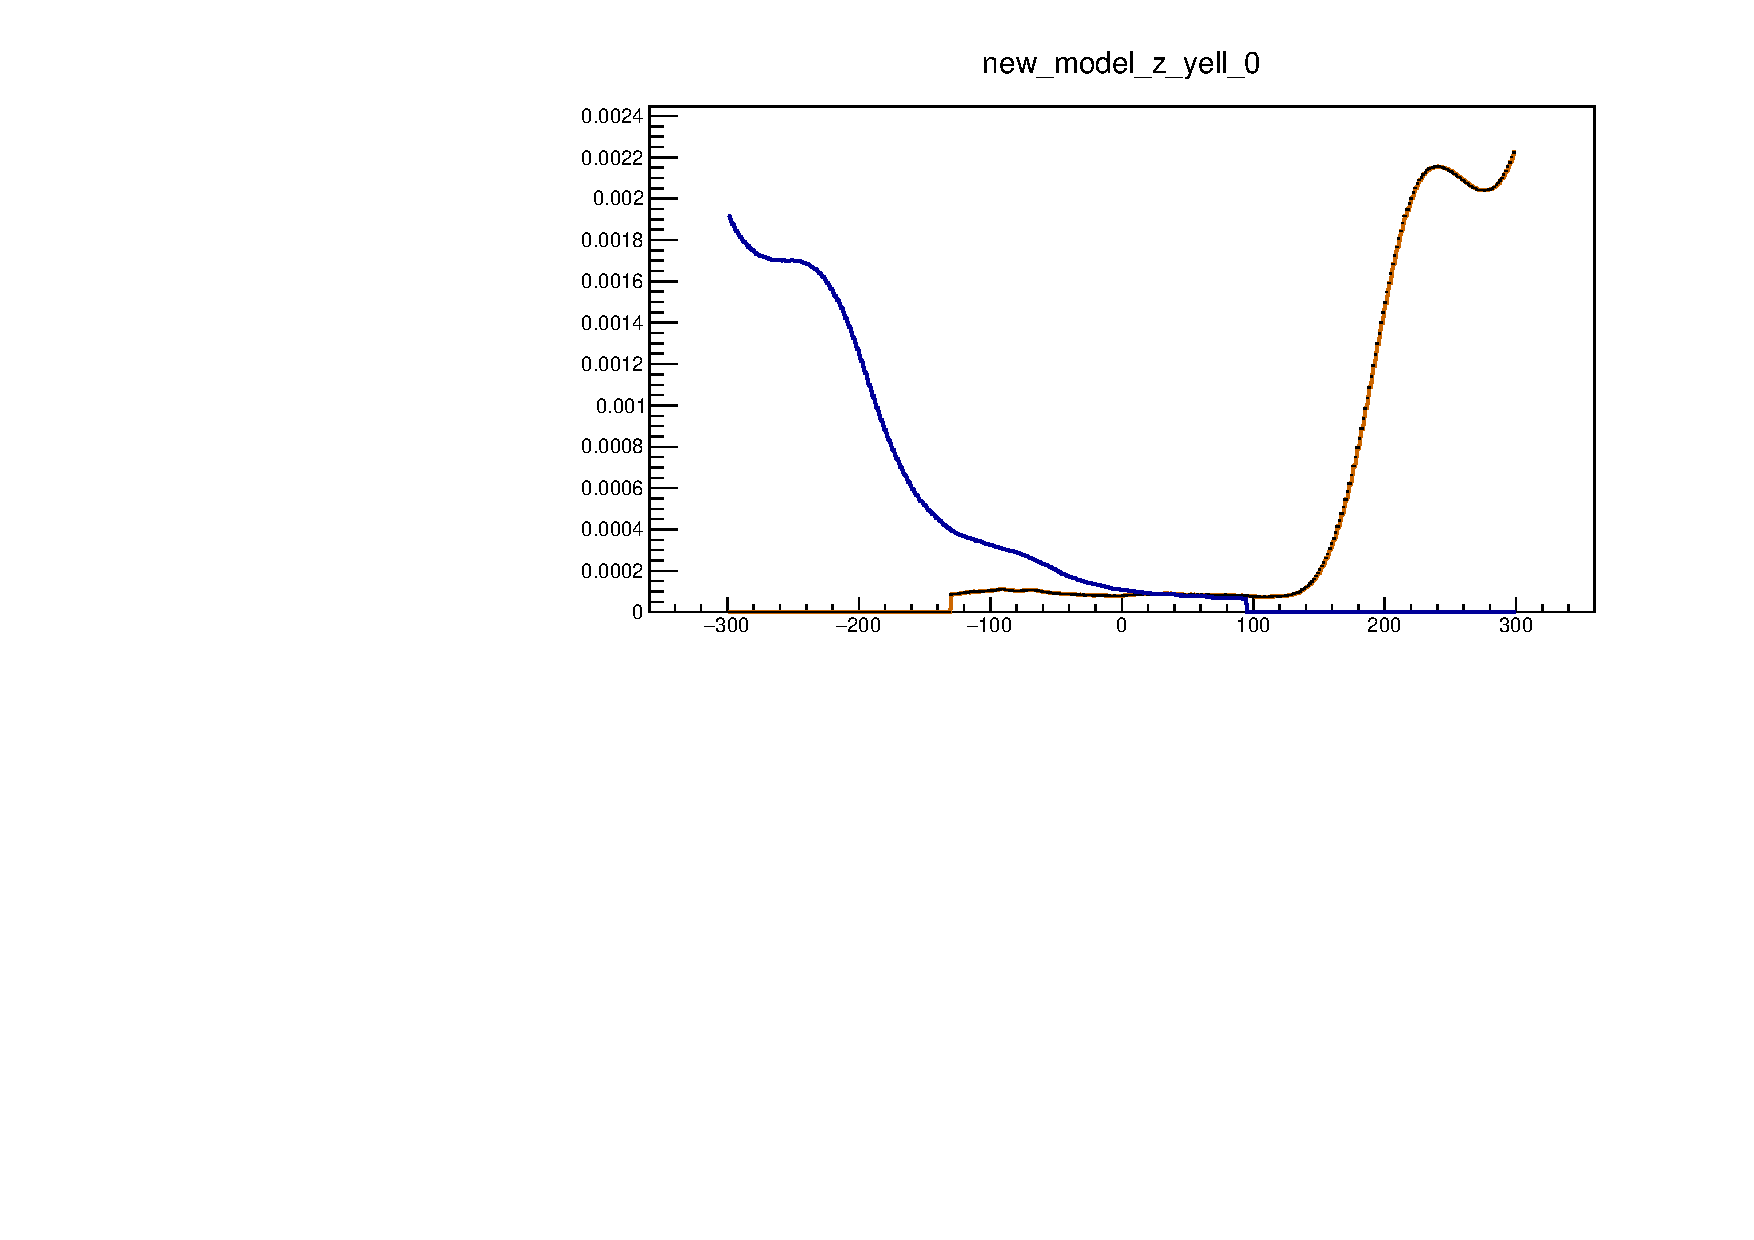
\includegraphics[width=0.8\linewidth]{../OverlapTest/figs/359711_time_step_0_bunch_collision.pdf}
\end{center}
\caption{Pictured here, we observe the blue and yellow bunches from a fixed
point in space (z = 0). Blue is incoming from the right, yellow, from the left.
The time resolution of the simulation is $\approx$2.5 ns. Shown: 12.5 ns before
collision }
\label{fig:359711_time_step_0_bunch_collision}
\end{figure}
\end{frame}

\begin{frame}{Do Bunches Collide Maximally Overlapped?}
\begin{figure}
\begin{center}
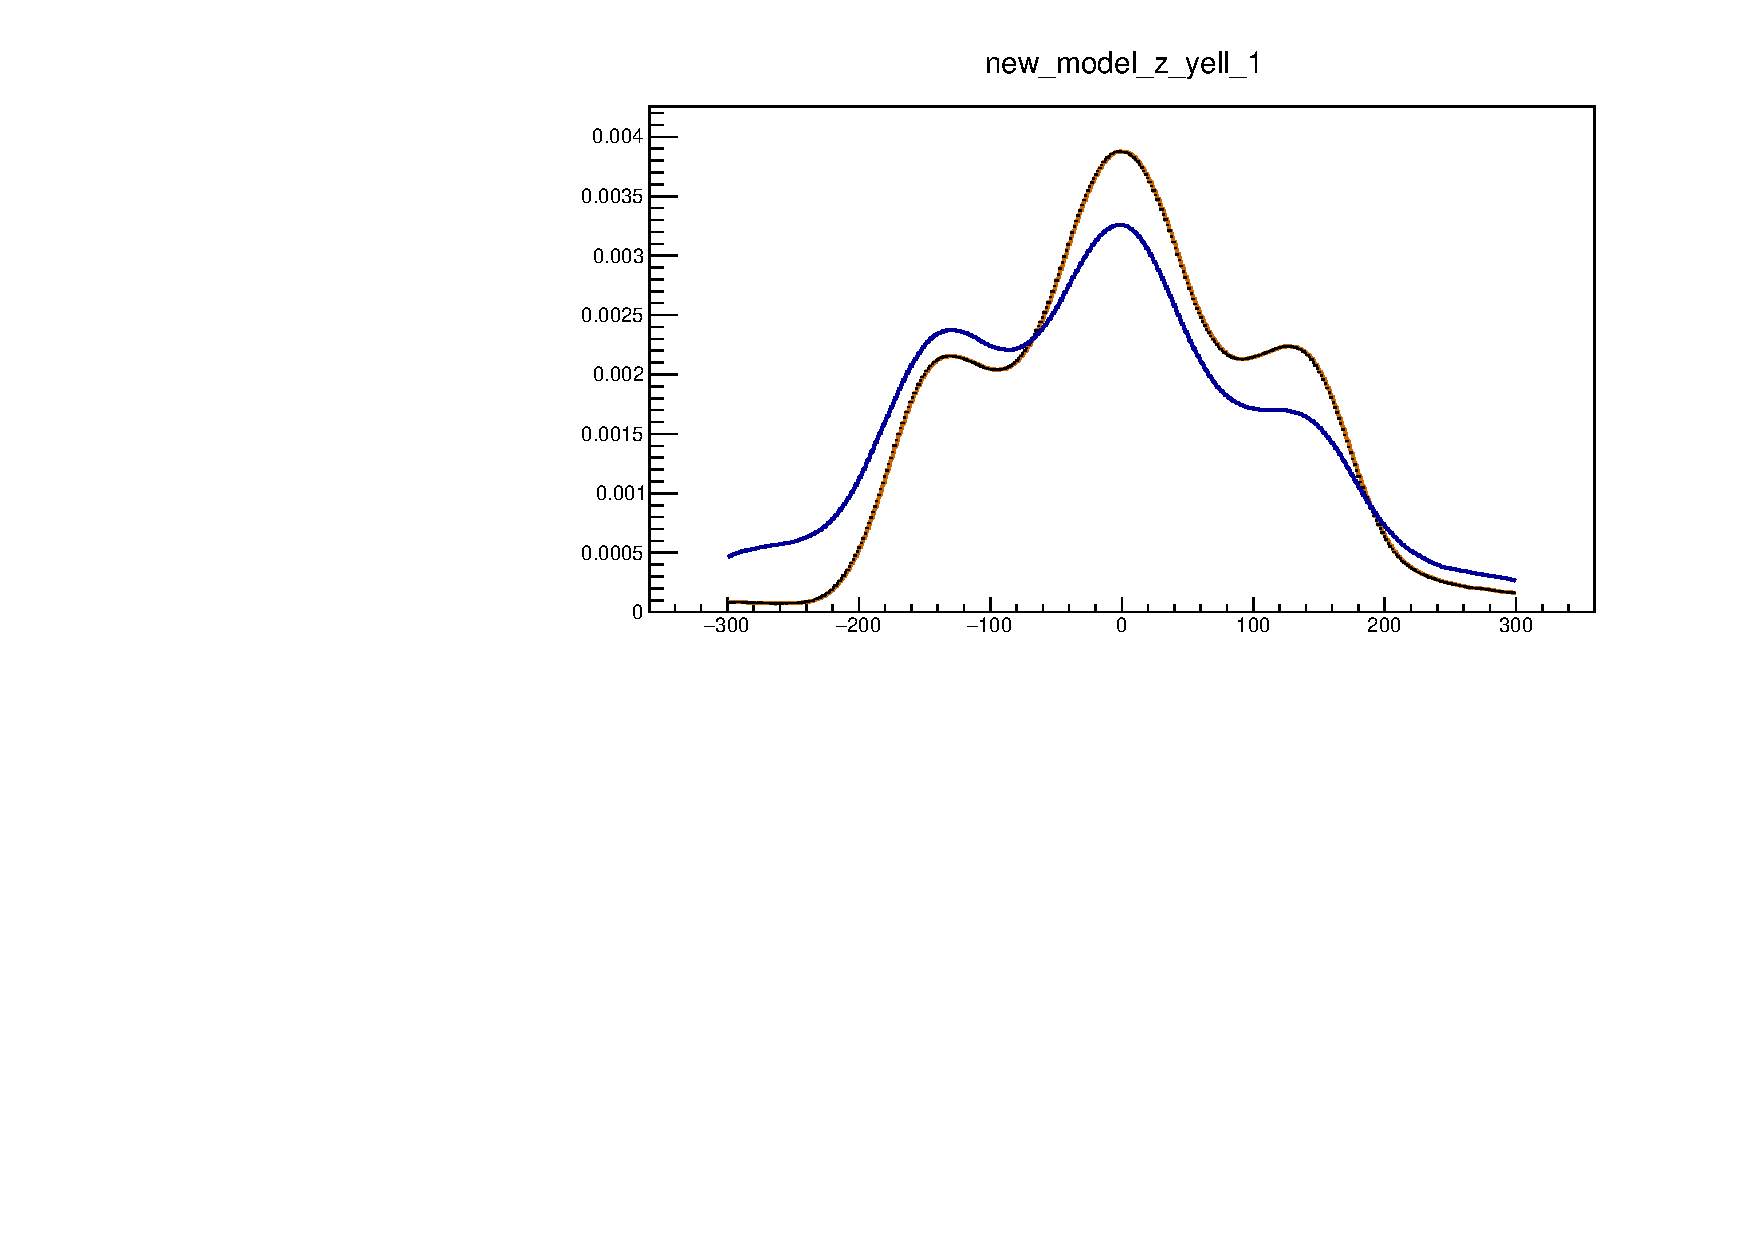
\includegraphics[width=0.8\linewidth]{../OverlapTest/figs/359711_time_step_1_bunch_collision.pdf}
\end{center}
\caption{Pictured here, we see the blue and yellow bunches at the nominal
interaction time, t = 0. The maxima of each bunch aligns exactly with z = 0.
Again, we observe from a fixed point in space, at z = 0. }
\label{fig:359711_time_step_1_bunch_collision}
\end{figure}
\end{frame}

\begin{frame}{Do Bunches Collide Maximally Overlapped?}
\begin{figure}
\begin{center}
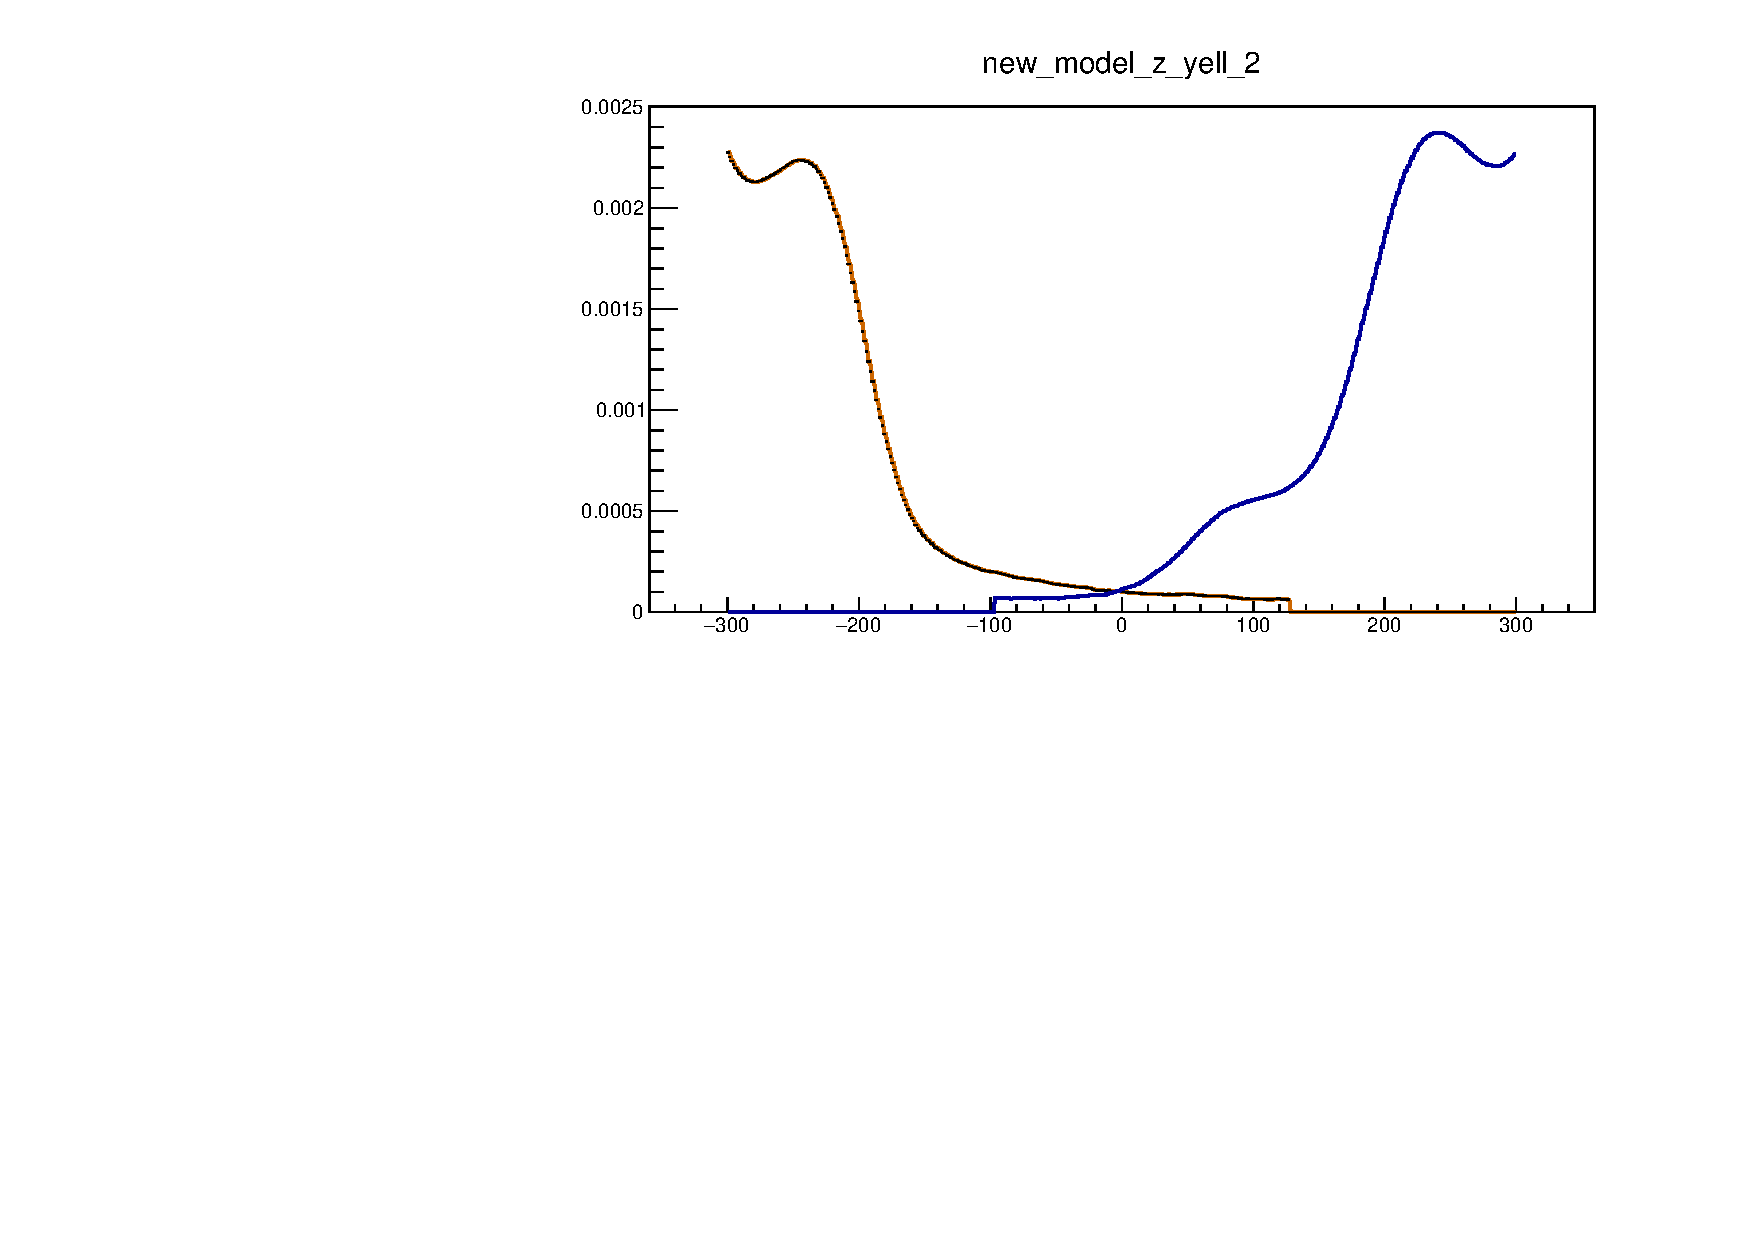
\includegraphics[width=0.8\linewidth]{../OverlapTest/figs/359711_time_step_2_bunch_collision.pdf}
\end{center}
\caption{Finally, we observe the bunches after the nominal interaction time,
from a fixed z-position. Another 12.5 ns have passed, and we can see the blue
bunch as continued to the right, and the yellow to the left.}
\label{fig:359711_time_step_2_bunch_collision}
\end{figure}
\end{frame}

\subsection{ WCM - Data vs Fit }
\begin{frame}
\frametitle{WCM Data Model, With Crossing Angle }
\begin{figure}
\begin{center}
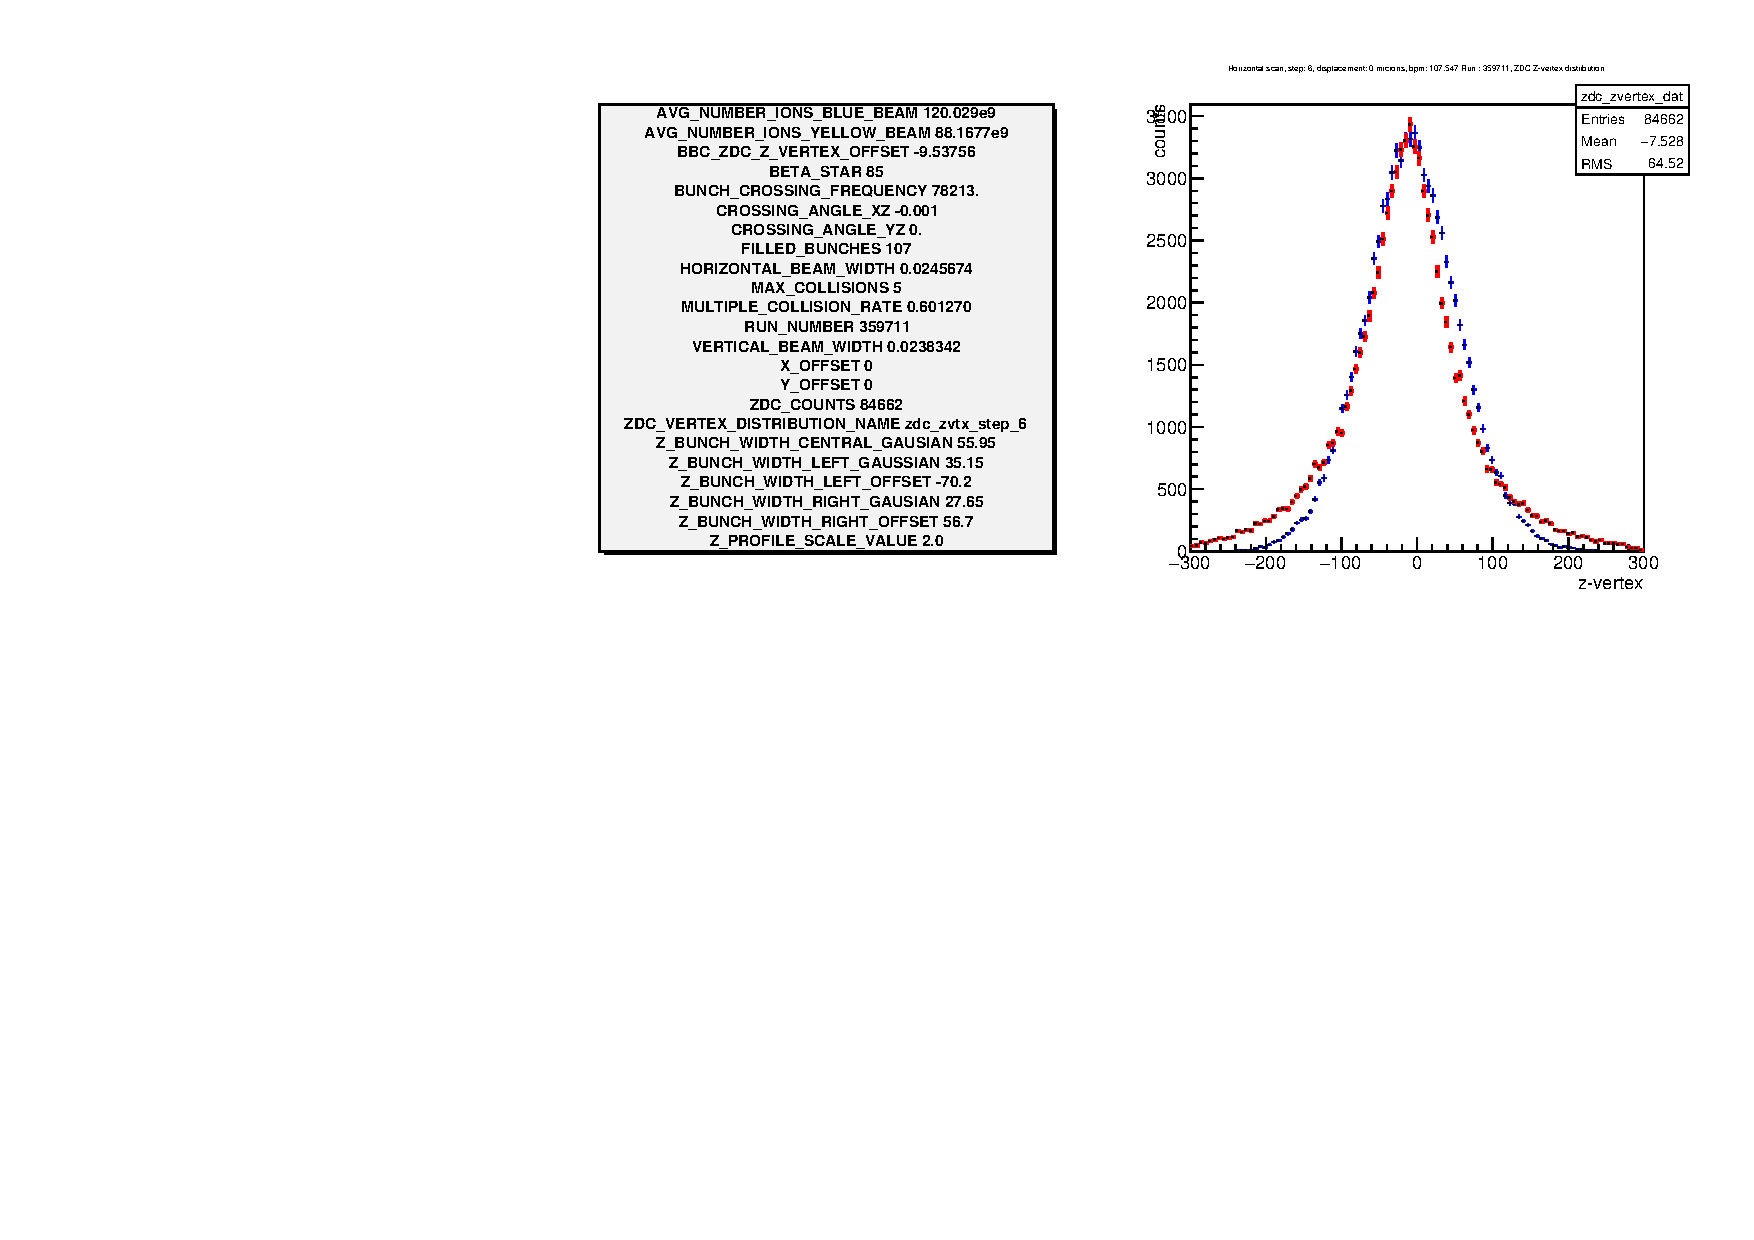
\includegraphics[width=\linewidth]{../OverlapTest/figs/359711_model0_angle_vertex.pdf}
\end{center}
\caption{This distriubtion is the result of my root-finding algorithm for
getting convergence, with some minor hand tuning. The non-zero crossing angle
makes the humped asymmetry disappear.}
\label{fig:359711_model0_angle_vertex}
\end{figure}
\end{frame}


\begin{frame}
\frametitle{WCM Data Model, With Crossing Angle }
\begin{figure}
\begin{center}
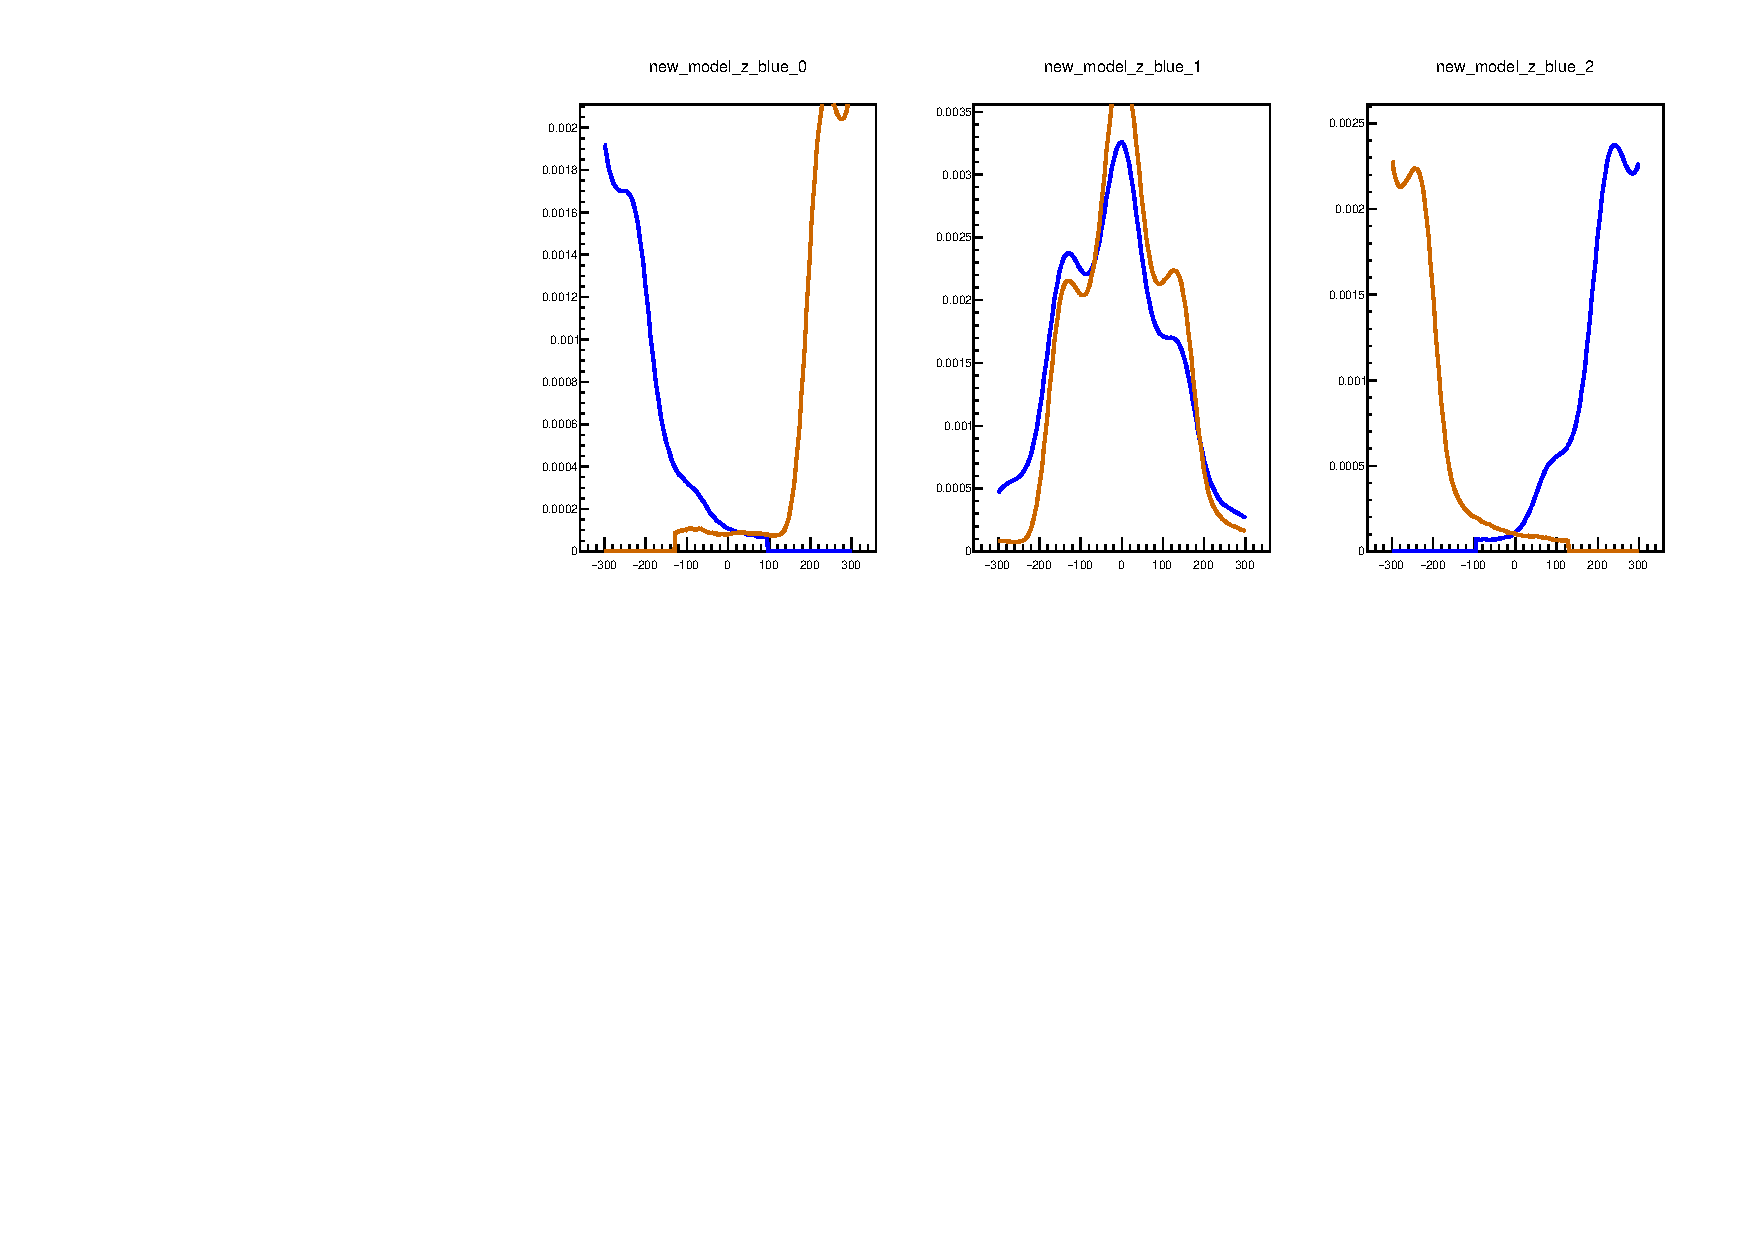
\includegraphics[width=\linewidth]{../OverlapTest/figs/359711_model0_angle_zprofile.pdf}
\end{center}
\caption{Snapshots of beam profiles as they collide, time increases from left to right }
\label{fig:359711_model0_angle_zprofile}
\end{figure}
\end{frame}


\begin{frame}
\frametitle{WCM Data Model, No Crossing Angle}
\begin{figure}
\begin{center}
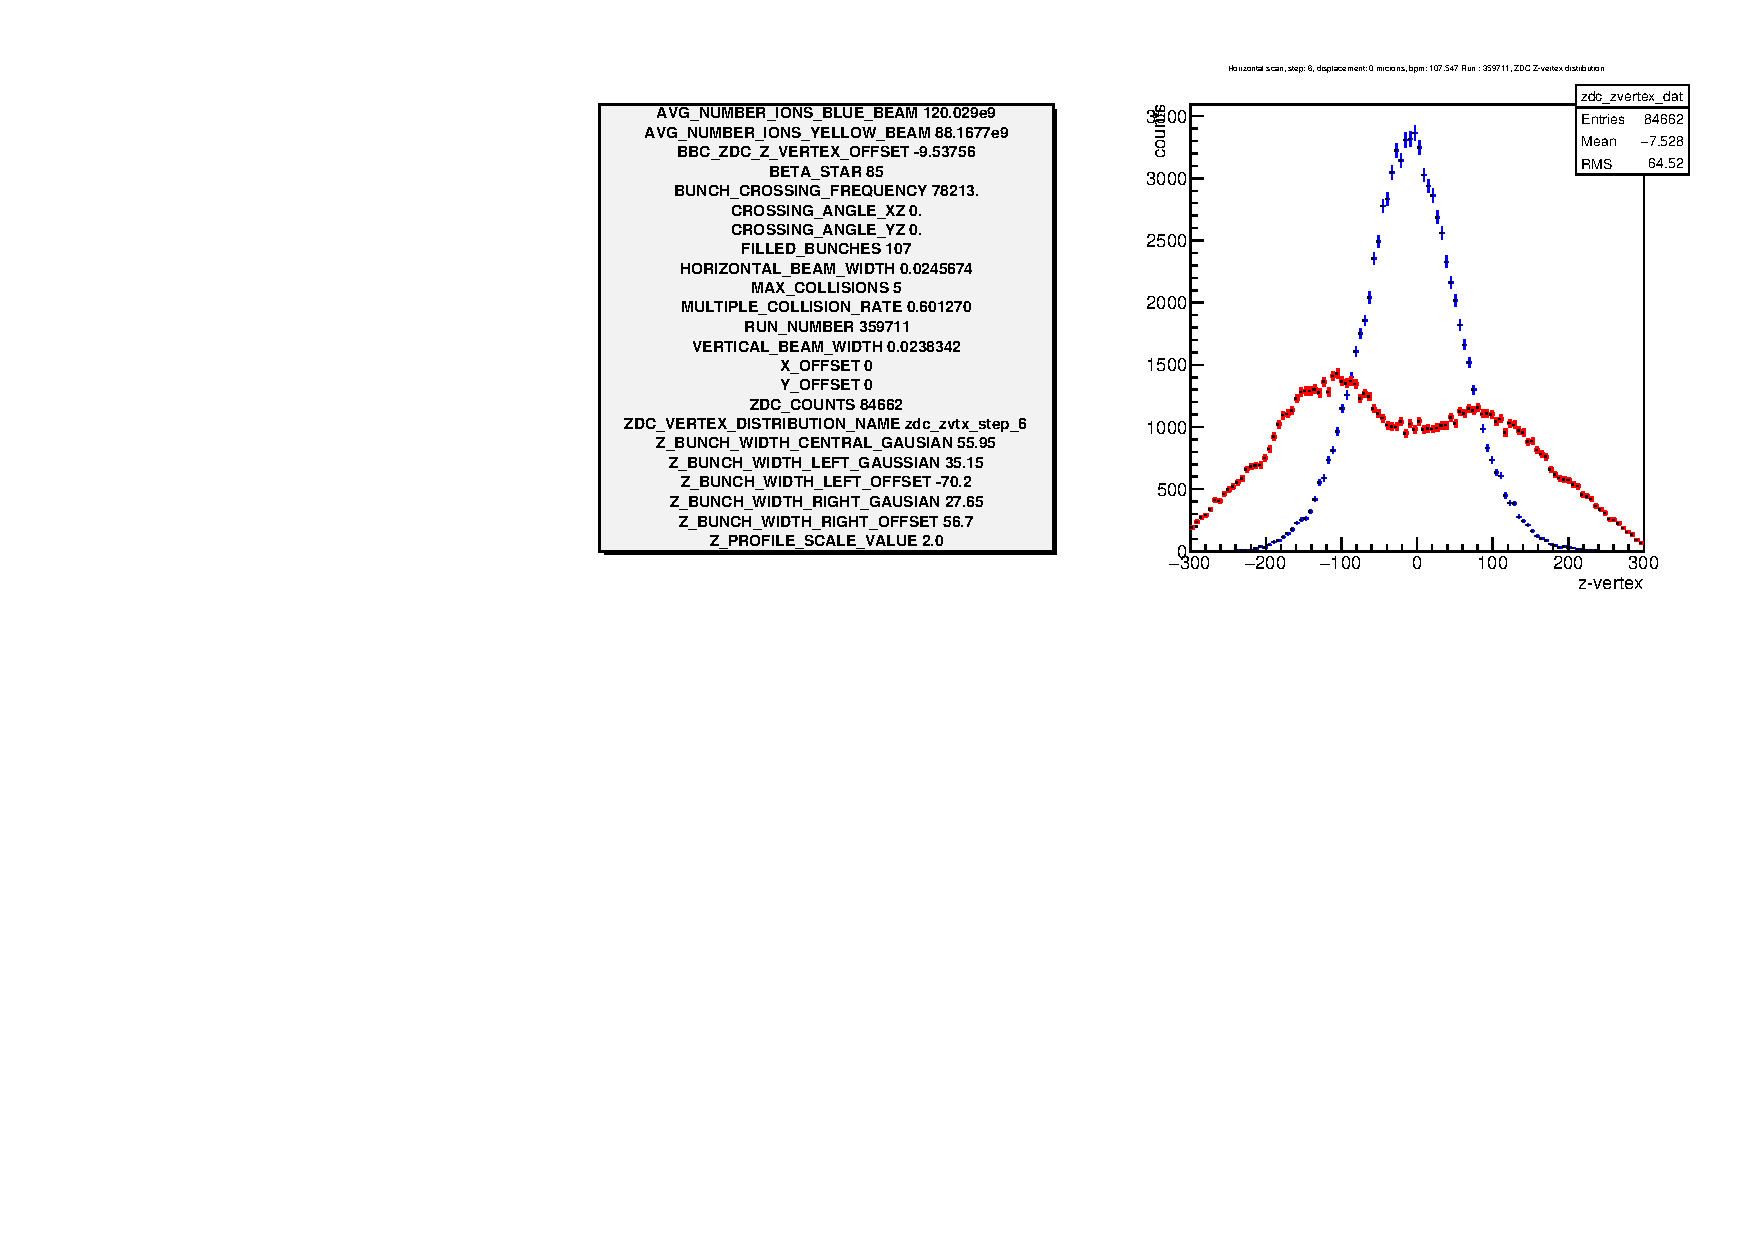
\includegraphics[width=\linewidth]{../OverlapTest/figs/359711_model0_noangle_vertex.pdf}
\end{center}
\caption{In the absense of a crossing angle, we see the max-overap peak split,
and the overall distriubtion widen, when using the WCM z-profile. }
\label{fig:359711_model0_noangle_vertex}
\end{figure}
\end{frame}


\begin{frame}
\frametitle{WCM Data Model, No Crossing Angle}
\begin{figure}
\begin{center}
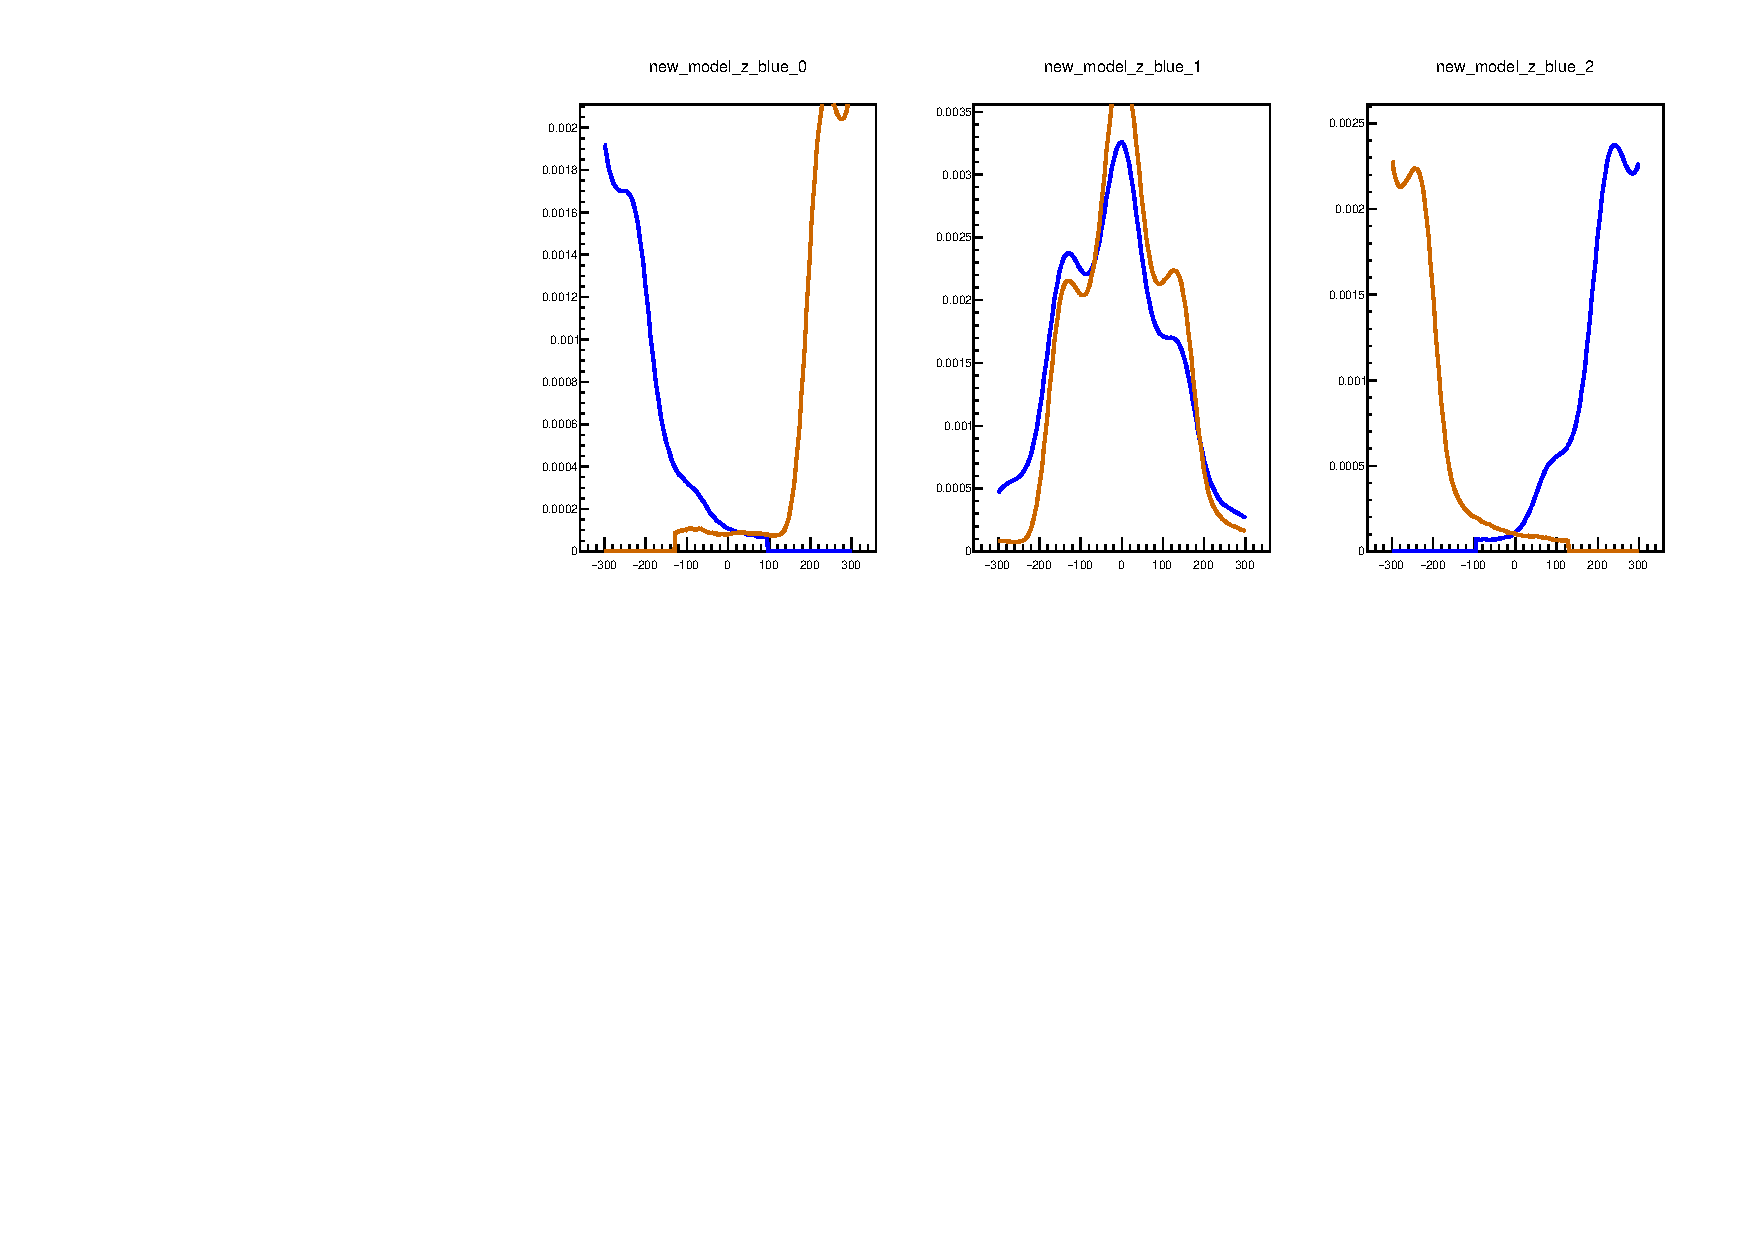
\includegraphics[width=\linewidth]{../OverlapTest/figs/359711_model0_noangle_zprofile.pdf}
\end{center}
\caption{Snapshots of beam profiles as they collide, time increases from left to right }
\label{fig:359711_model0_noangle_zprofile}
\end{figure}
\end{frame}


\begin{frame}
\frametitle{WCM Data Model, Triple Gaussian Fit, With Crossing Angle}
\begin{figure}
\begin{center}
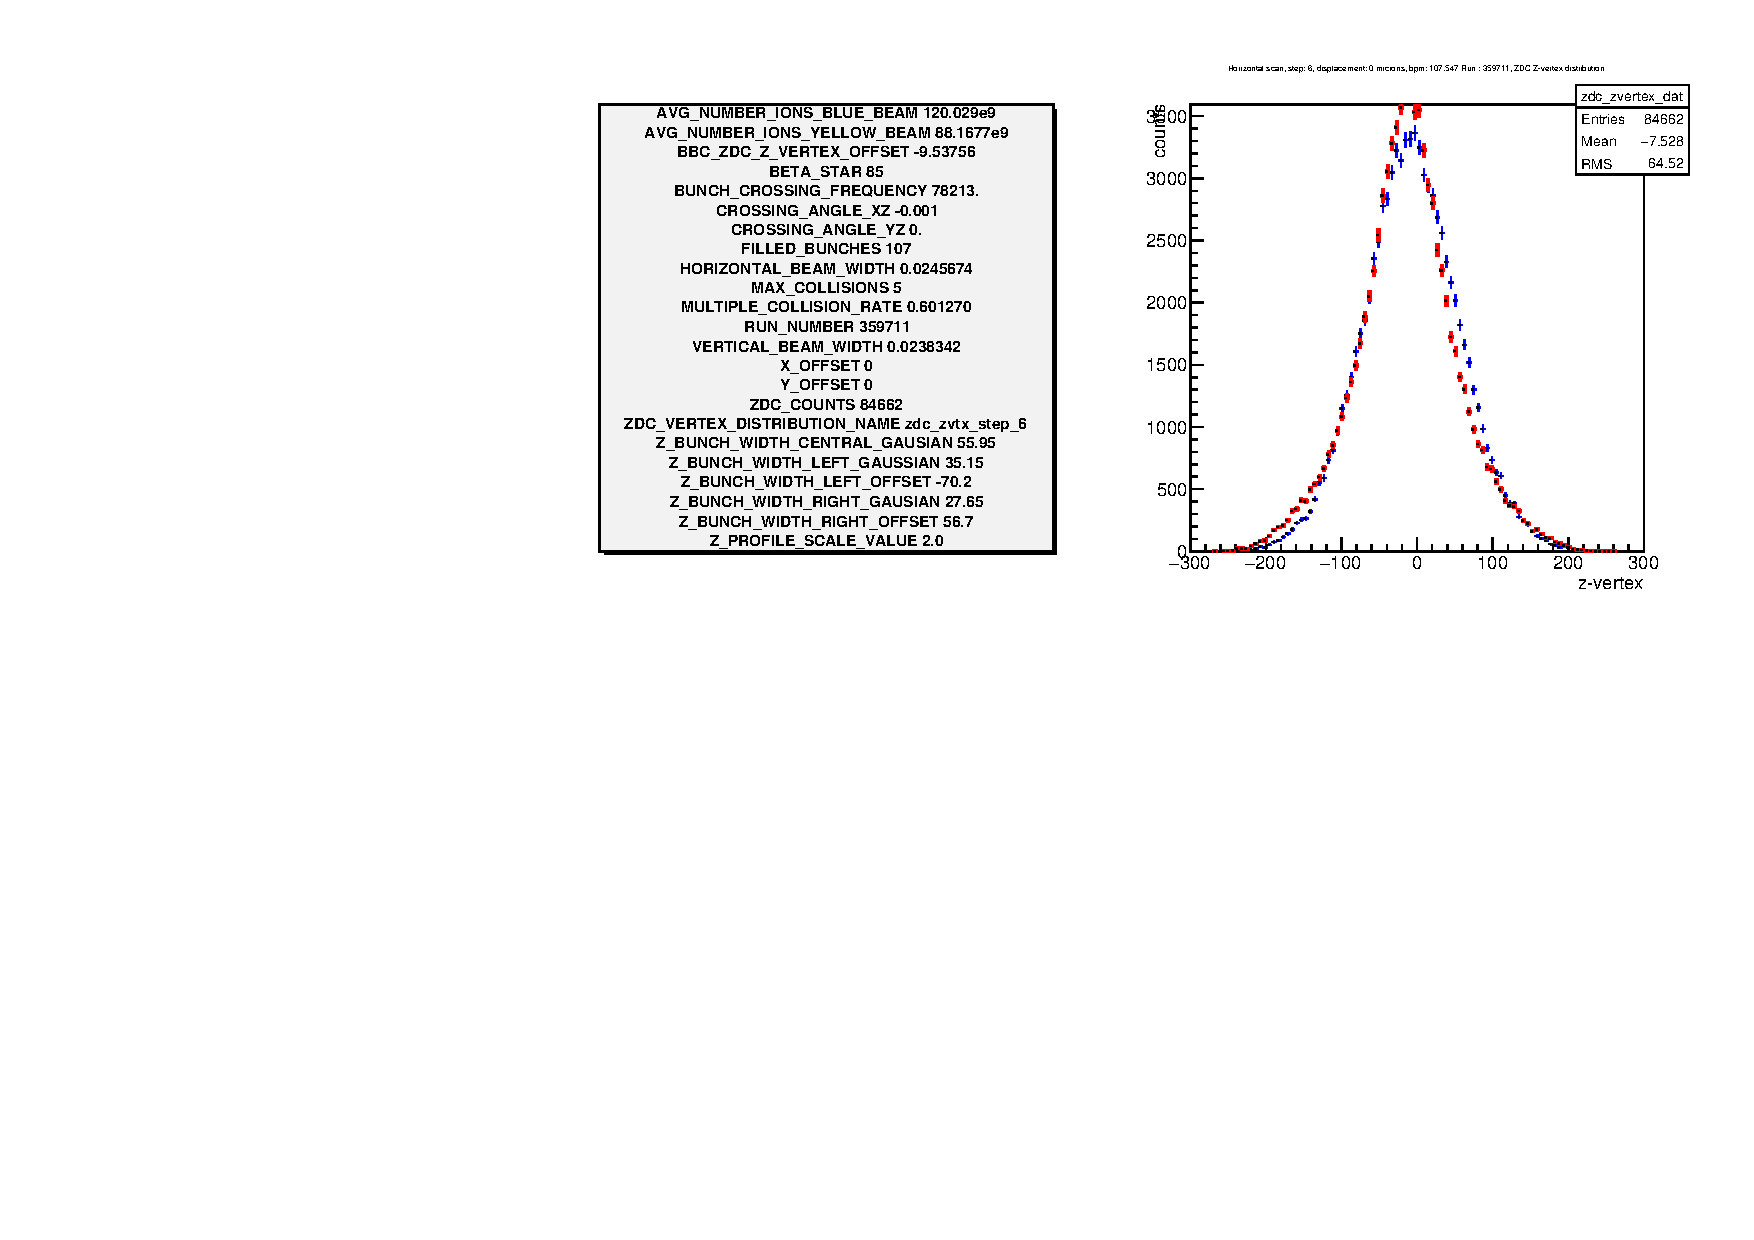
\includegraphics[width=\linewidth]{../OverlapTest/figs/359711_model2_angle_vertex.pdf}
\end{center}
\caption{More or less similar shape to the WCM data. Using a fit for the
z-profile cuts out any edge effects.}
\label{fig:359711_model2_angle_vertex}
\end{figure}
\end{frame}


\begin{frame}
\frametitle{WCM Data Model, Triple Gaussian Fit, With Crossing Angle}
\begin{figure}
\begin{center}
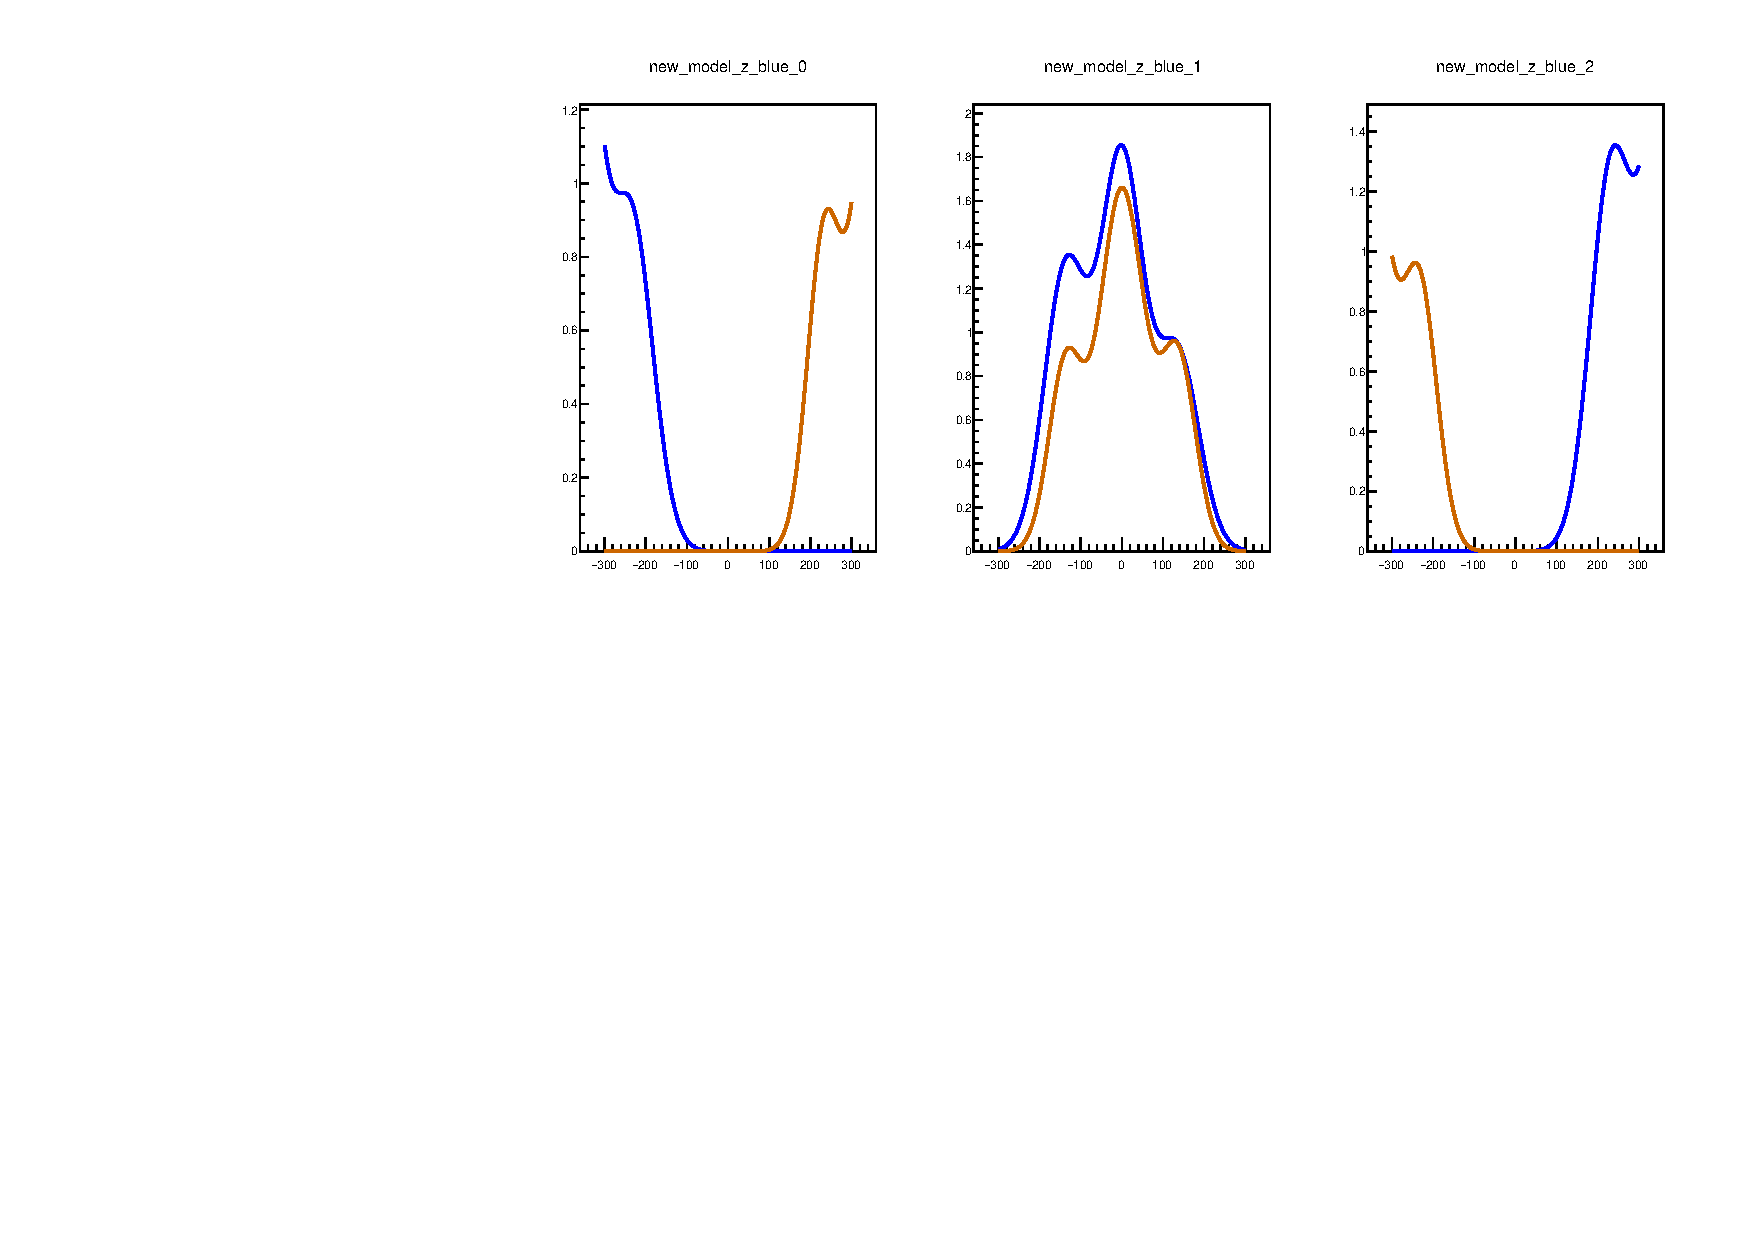
\includegraphics[width=\linewidth]{../OverlapTest/figs/359711_model2_angle_zprofile.pdf}
\end{center}
\caption{Snapshots of beam profiles as they collide, time increases from left to
right. Note the smooth edges of the beam profiles, as opposed to the rough
edges obtained from data. }
\label{fig:359711_model2_angle_zprofile}
\end{figure}
\end{frame}


\begin{frame}
\frametitle{WCM Data Model, Triple Gaussian Fit, No Crossing Angle}
\begin{figure}
\begin{center}
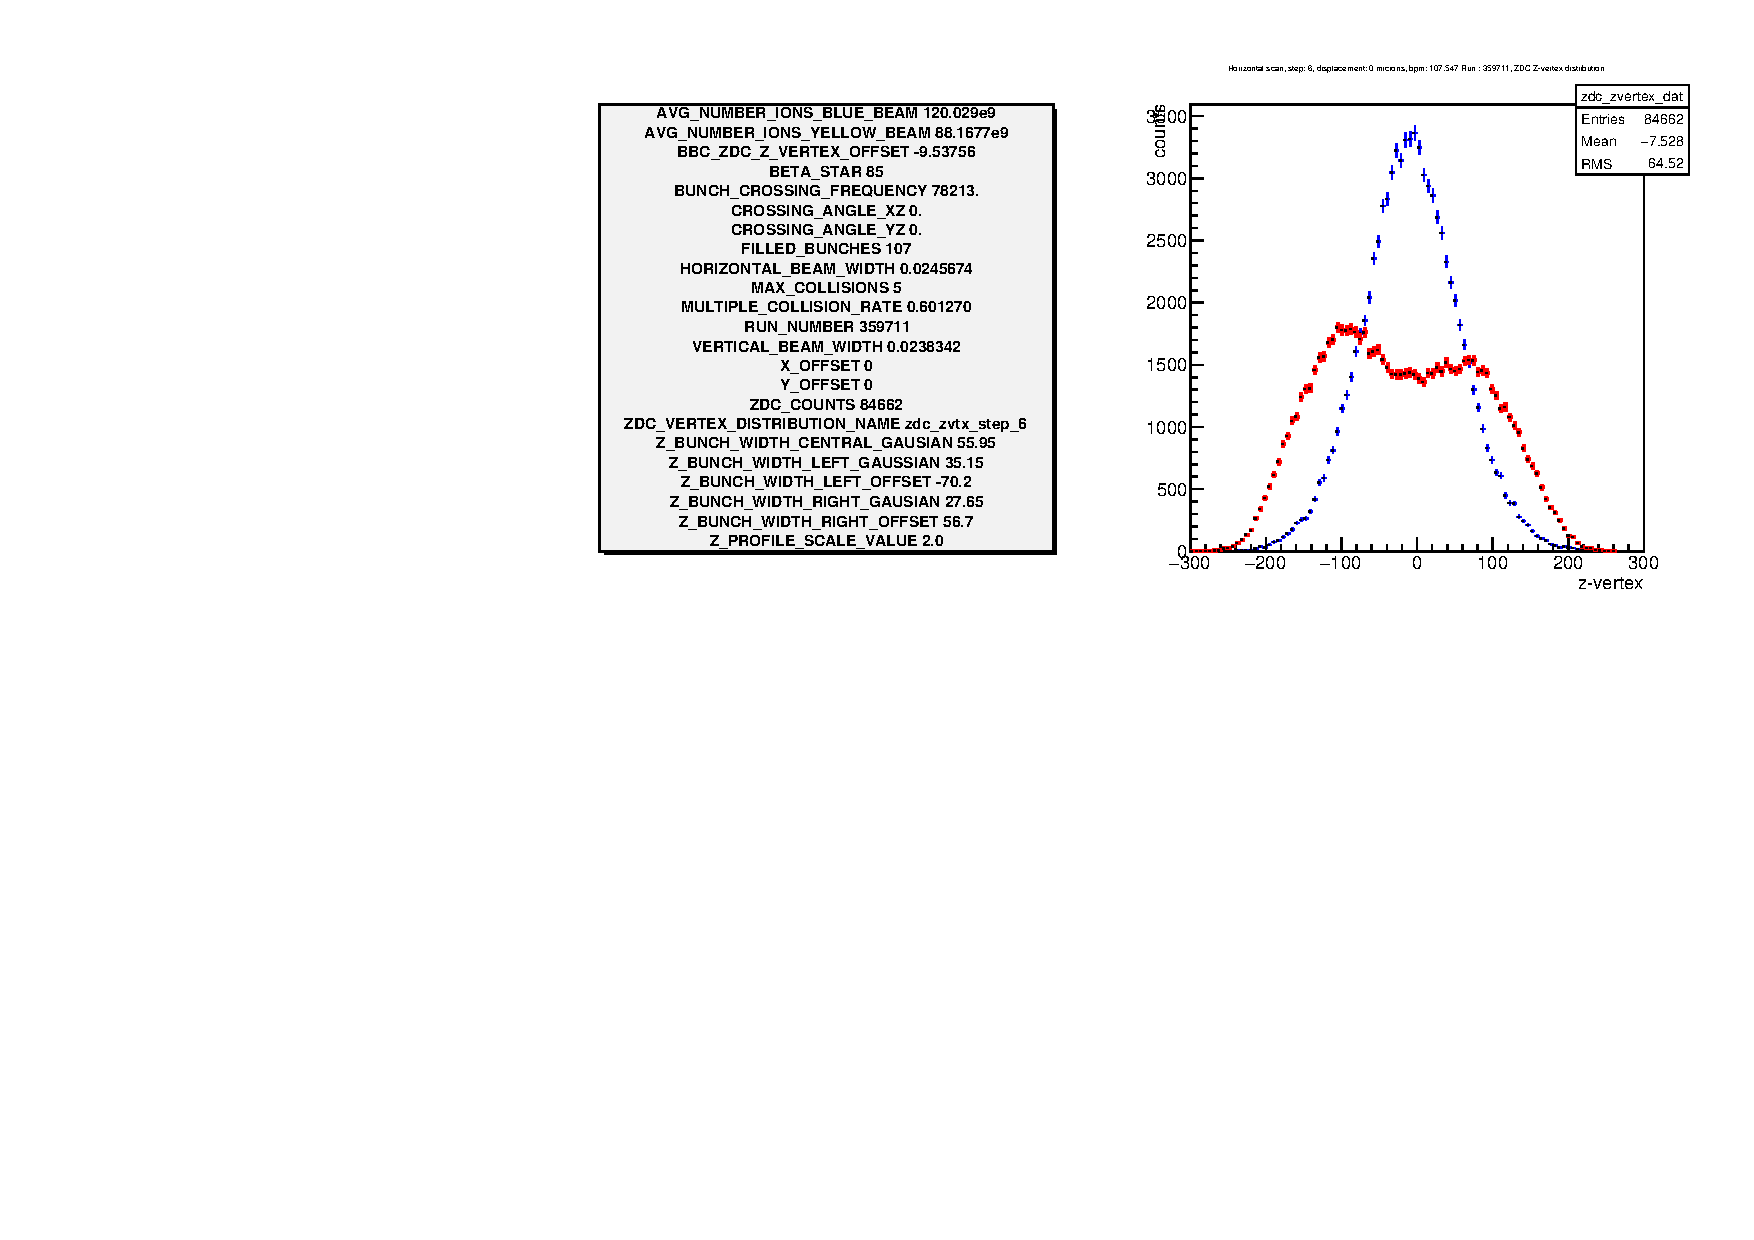
\includegraphics[width=\linewidth]{../OverlapTest/figs/359711_model2_noangle_vertex.pdf}
\end{center}
\caption{Similar behavior in the z-vertex distribution appears when we remove
the crossing angle.}
\label{fig:359711_model2_noangle_vertex}
\end{figure}
\end{frame}


\begin{frame}
\frametitle{WCM data Model, Triple Gaussian Fit, No Crossing Angle}
\begin{figure}
\begin{center}
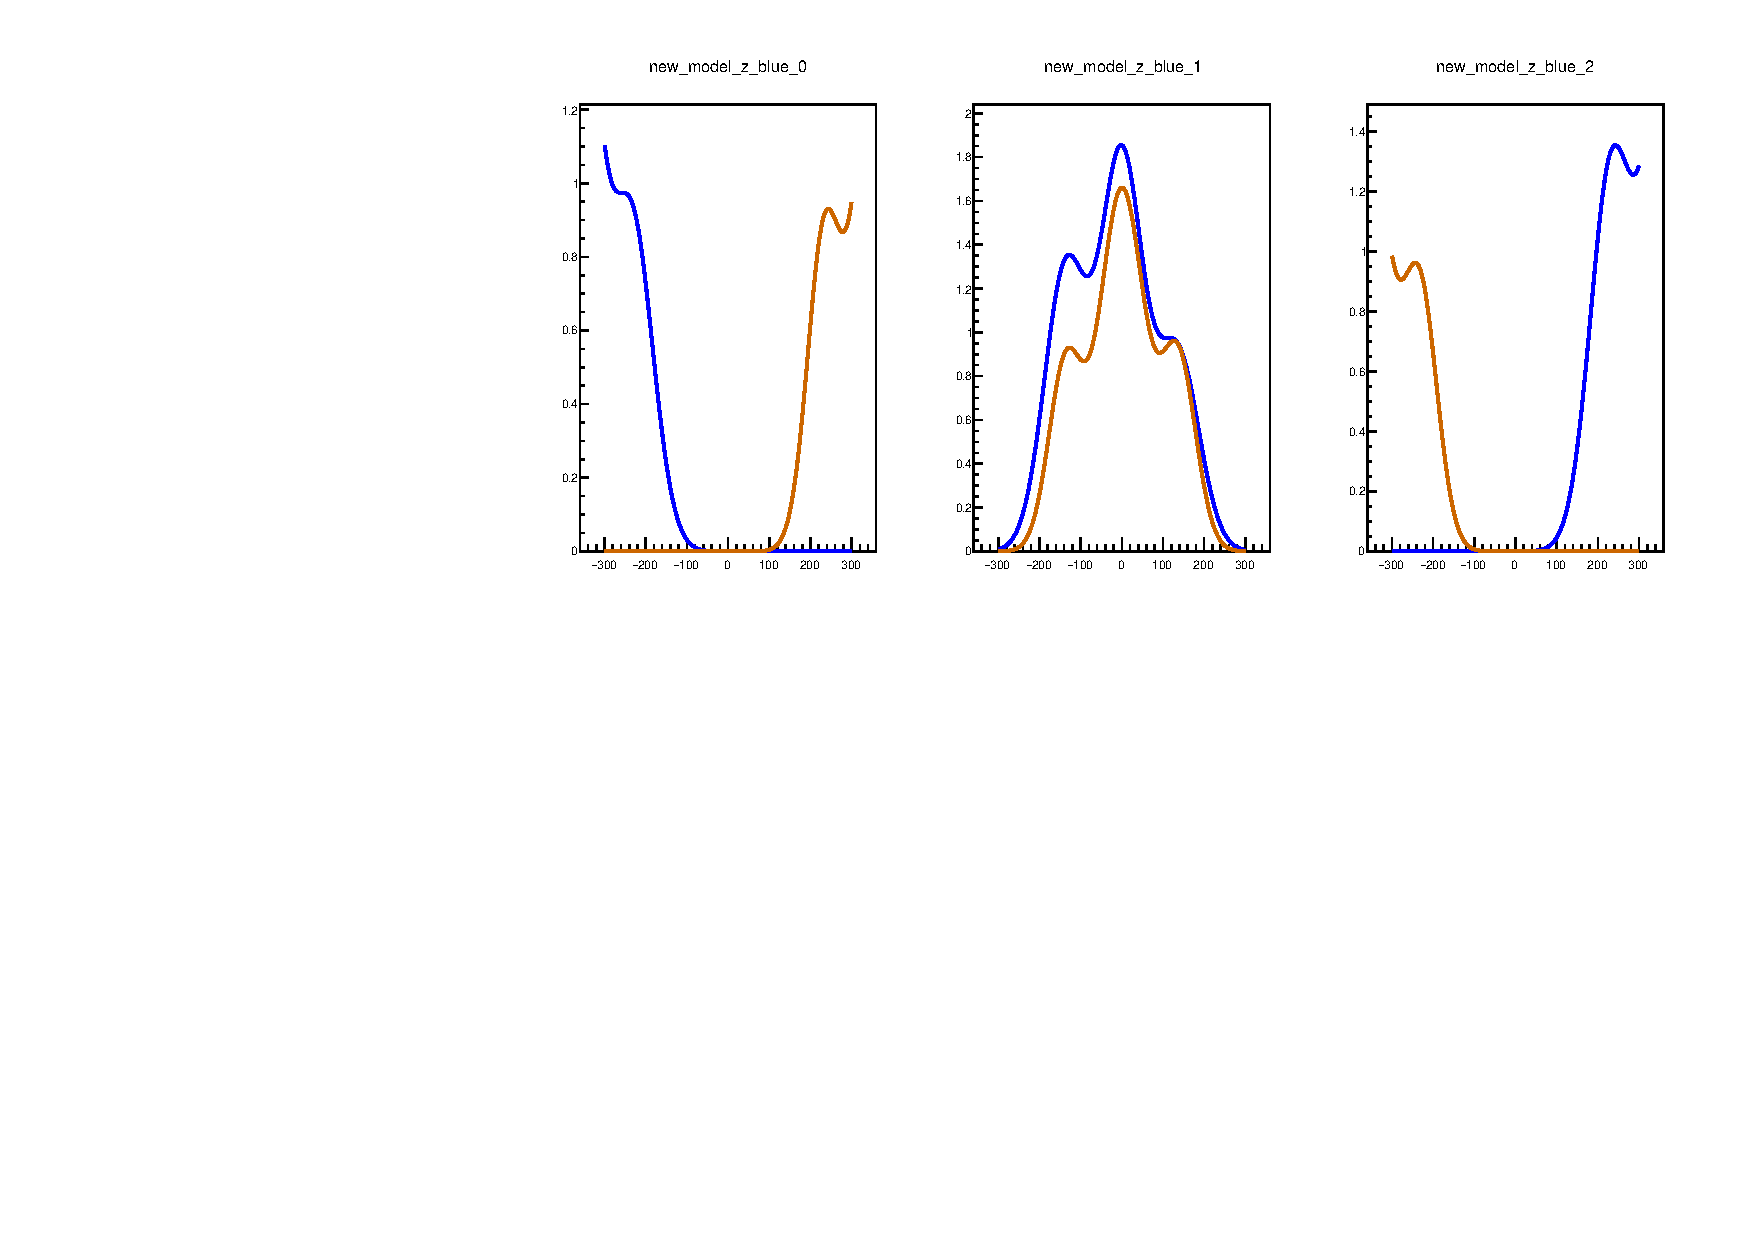
\includegraphics[width=\linewidth]{../OverlapTest/figs/359711_model2_noangle_zprofile.pdf}
\end{center}
\caption{Snapshots of beam profiles as they collide, time increases from left to right }
\label{fig:359711_model2_noangle_zprofile}
\end{figure}
\end{frame}


\subsection{ Amaresh's Triple Gaussian (via Run 15 Simulations) }
\begin{frame}
\frametitle{Amaresh Model, Left + Center + Right Gaussian, No Crossing Angle }
\begin{figure}
\begin{center}
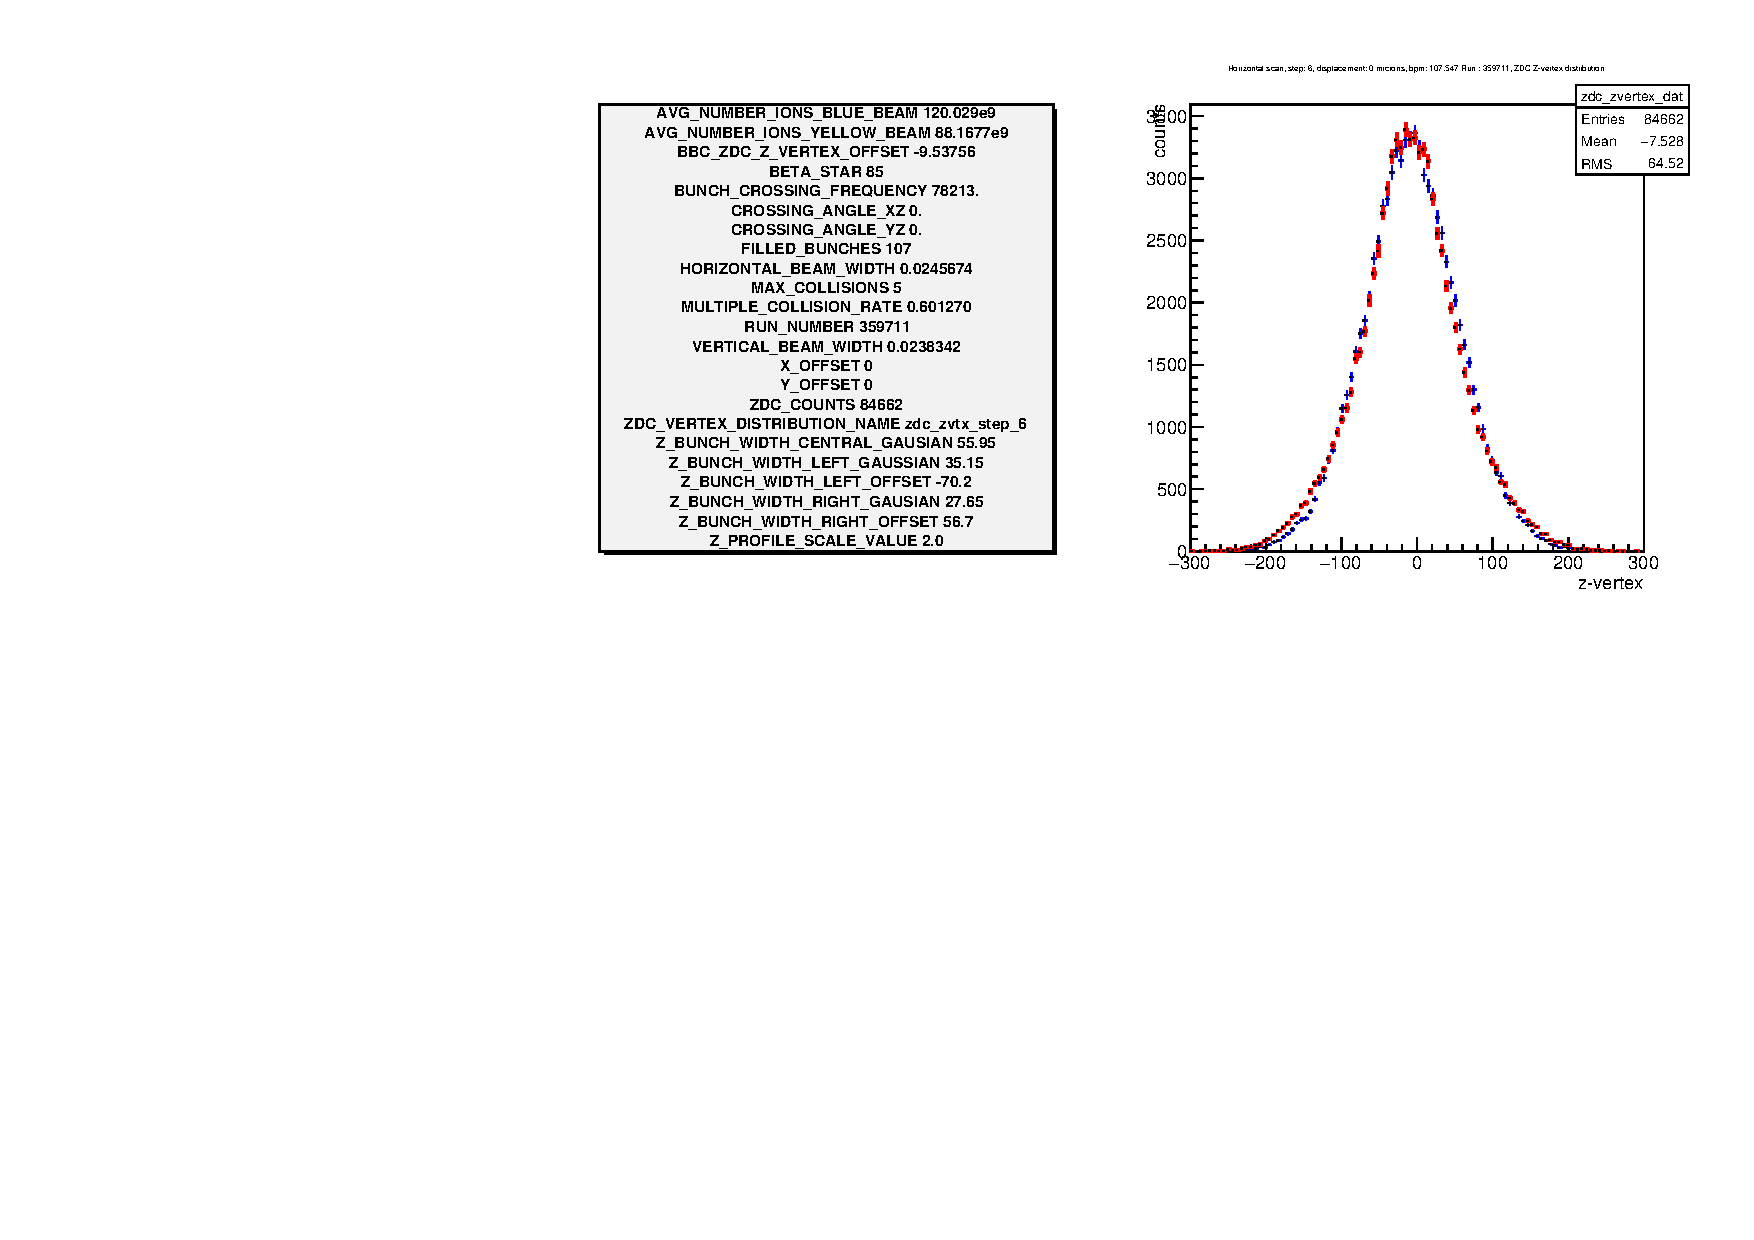
\includegraphics[width=\linewidth]{../OverlapTest/figs/359711_model1_angle_vertex.pdf}
\end{center}
\caption{The Amaresh model seems to converge at max-overlap very nicely, but
note that in this case, convergence is good without a crossing angle. }
\label{fig:359711_model1_angle_vertex}
\end{figure}
\end{frame}


\begin{frame}
\frametitle{Amaresh Model, Left + Center + Right Gaussian, No Crossing Angle }
\begin{figure}
\begin{center}
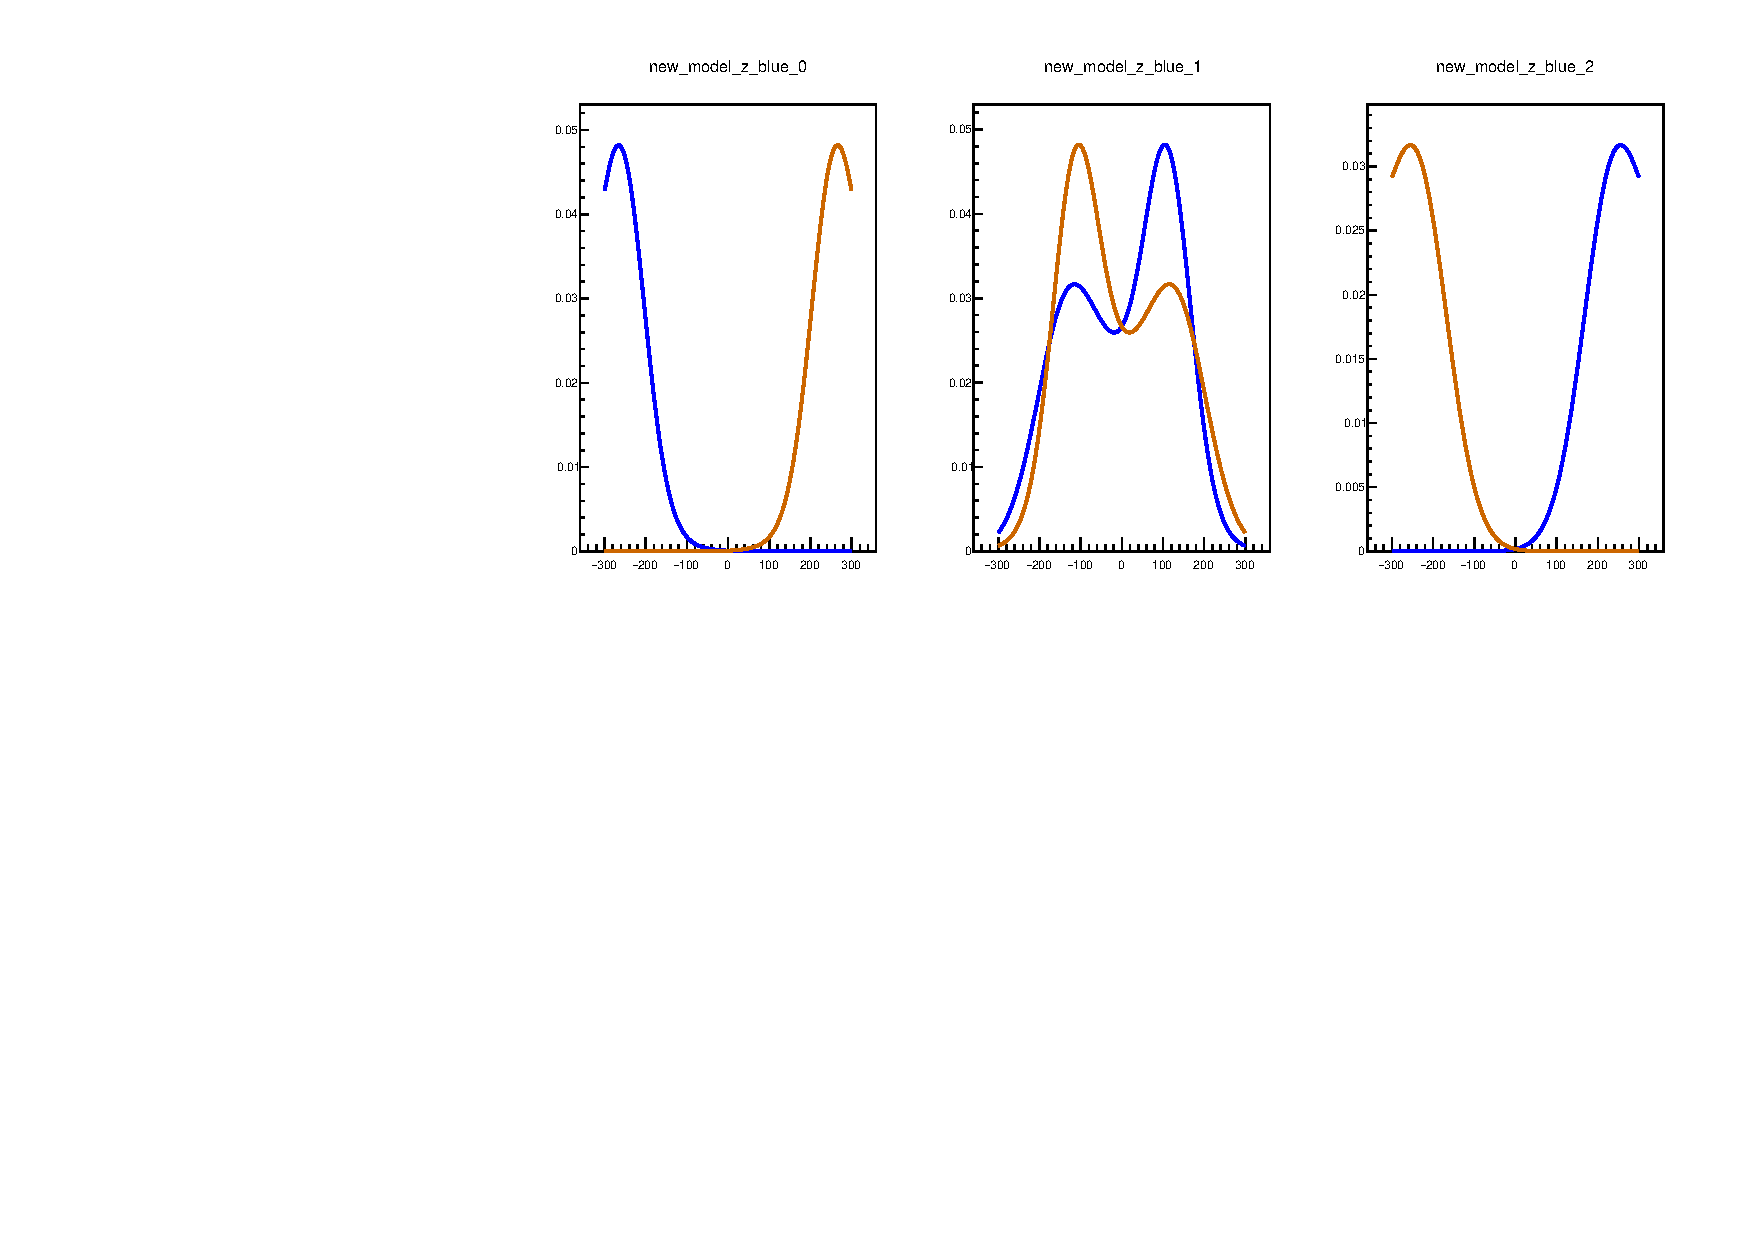
\includegraphics[width=\linewidth]{../OverlapTest/figs/359711_model1_angle_zprofile.pdf}
\end{center}
\caption{Snapshots of beam profiles as they collide, time increases from left to right }
\label{fig:359711_model1_angle_zprofile}
\end{figure}
\end{frame}



\begin{frame}
\frametitle{Amaresh Model, Central Gaussian Only, With Crossing Angle }
\begin{figure}
\begin{center}
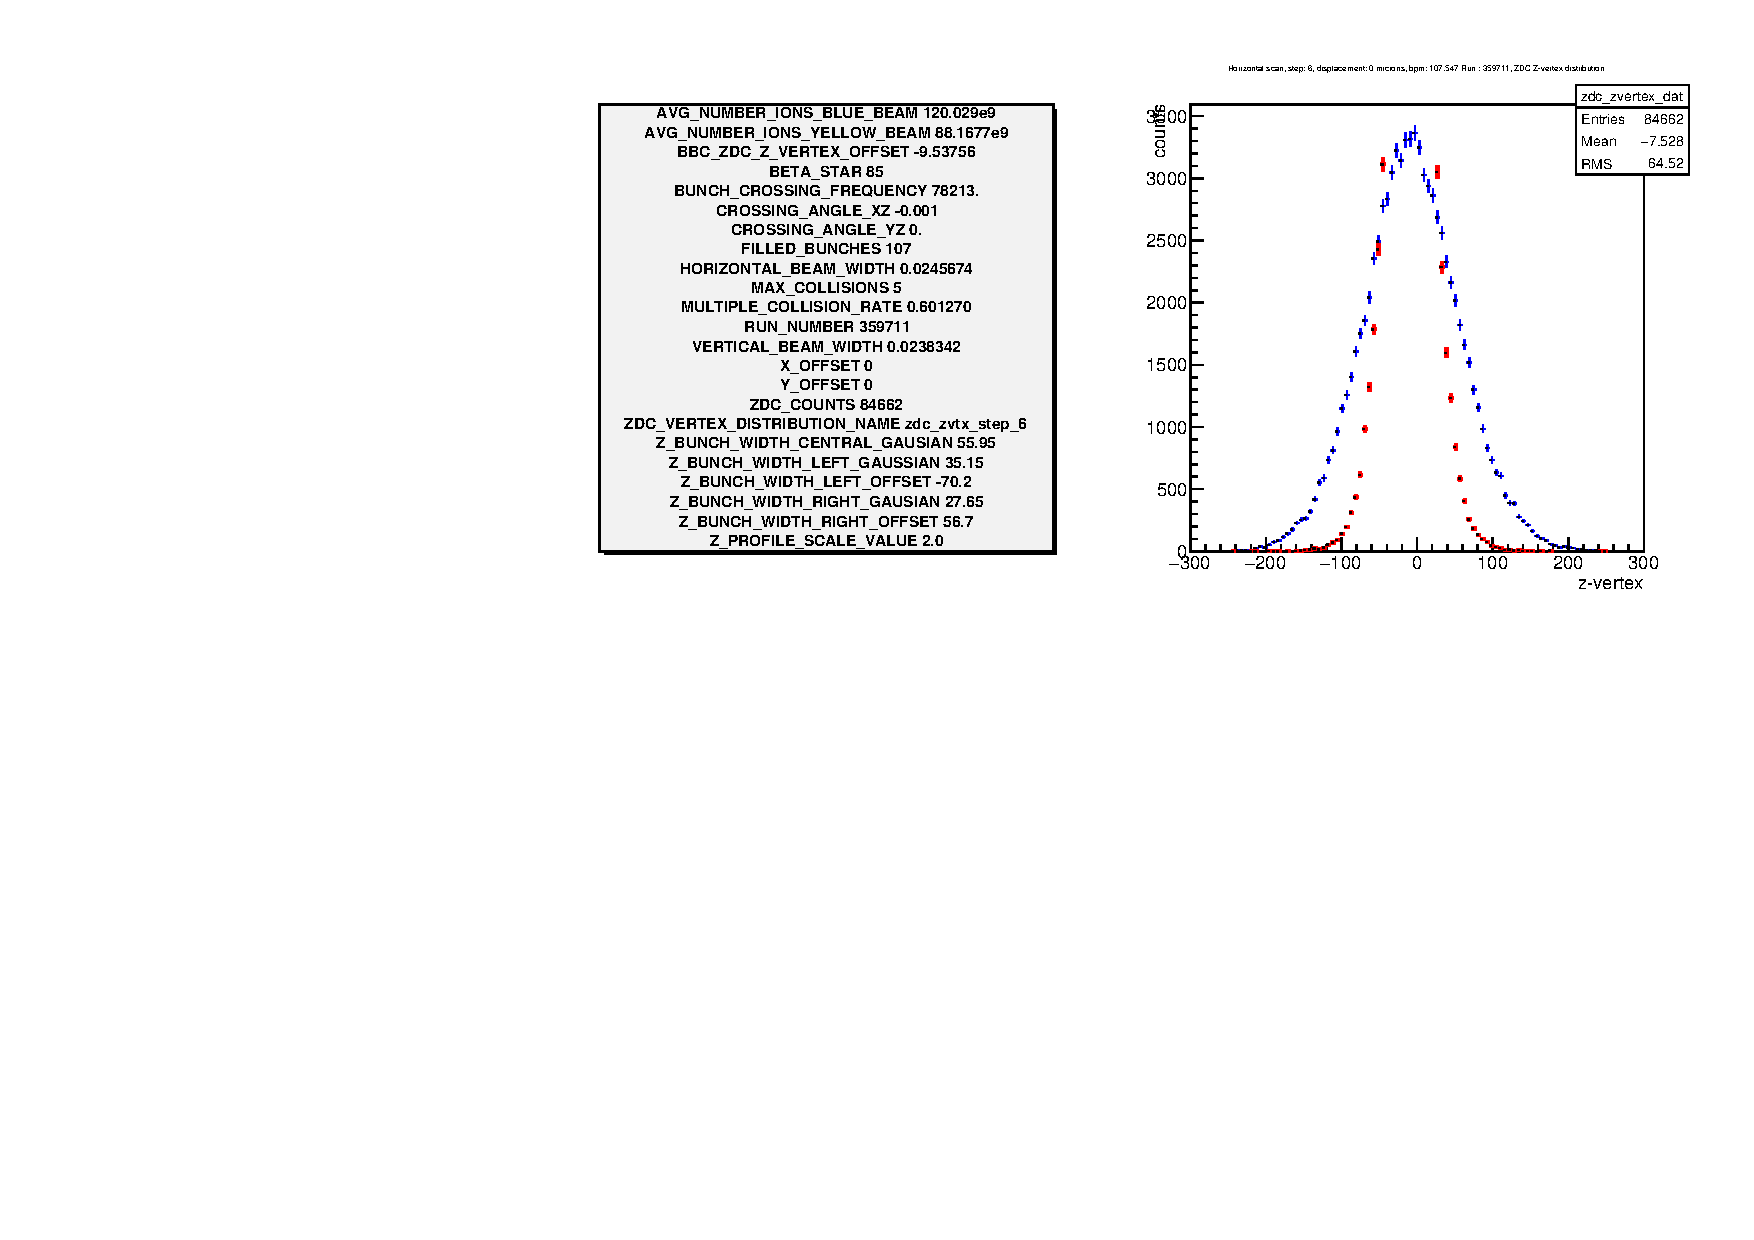
\includegraphics[width=\linewidth]{../OverlapTest/figs/359711_model0c_angle_vertex.pdf}
\end{center}
\caption{Here, we test if we see similar behavior from Amaresh's model if we
omit everything but the central gaussian from the z-profile. Matching becomes
bad.}
\label{fig:359711_model0c_angle_vertex}
\end{figure}
\end{frame}


\begin{frame}
\frametitle{Amaresh Model, Central Gaussian Only, With Crossing Angle }
\begin{figure}
\begin{center}
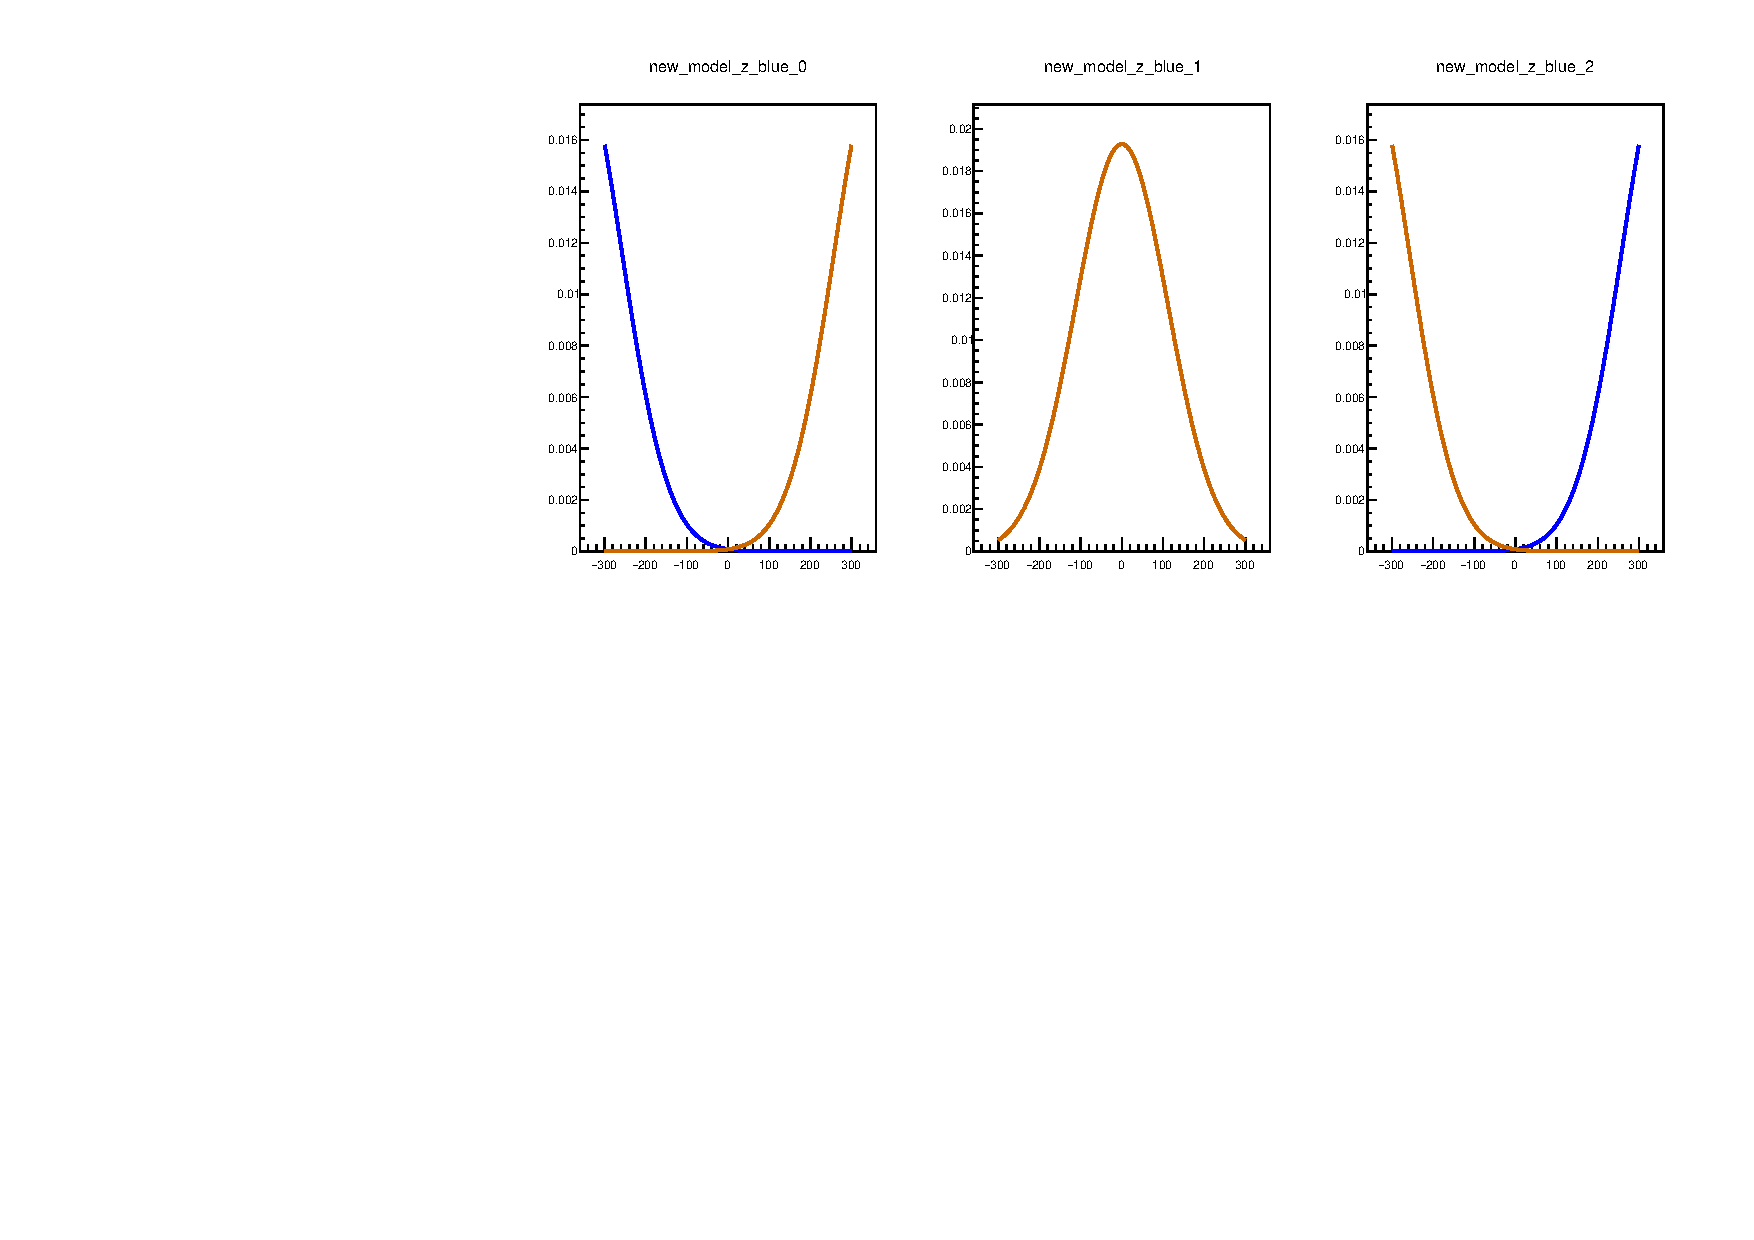
\includegraphics[width=\linewidth]{../OverlapTest/figs/359711_model0c_angle_zprofile.pdf}
\end{center}
\caption{Snapshots of beam profiles as they collide, time increases from left to
right. This also serves to confirm that while Amaresh's model is asymmetric, the
"center" of the distriubtions cross at z = 0}
\label{fig:359711_model0c_angle_zprofile}
\end{figure}
\end{frame}

\begin{frame}
\frametitle{Amaresh Model, Central Gaussian Only, No Crossing Angle }
\begin{figure}
\begin{center}
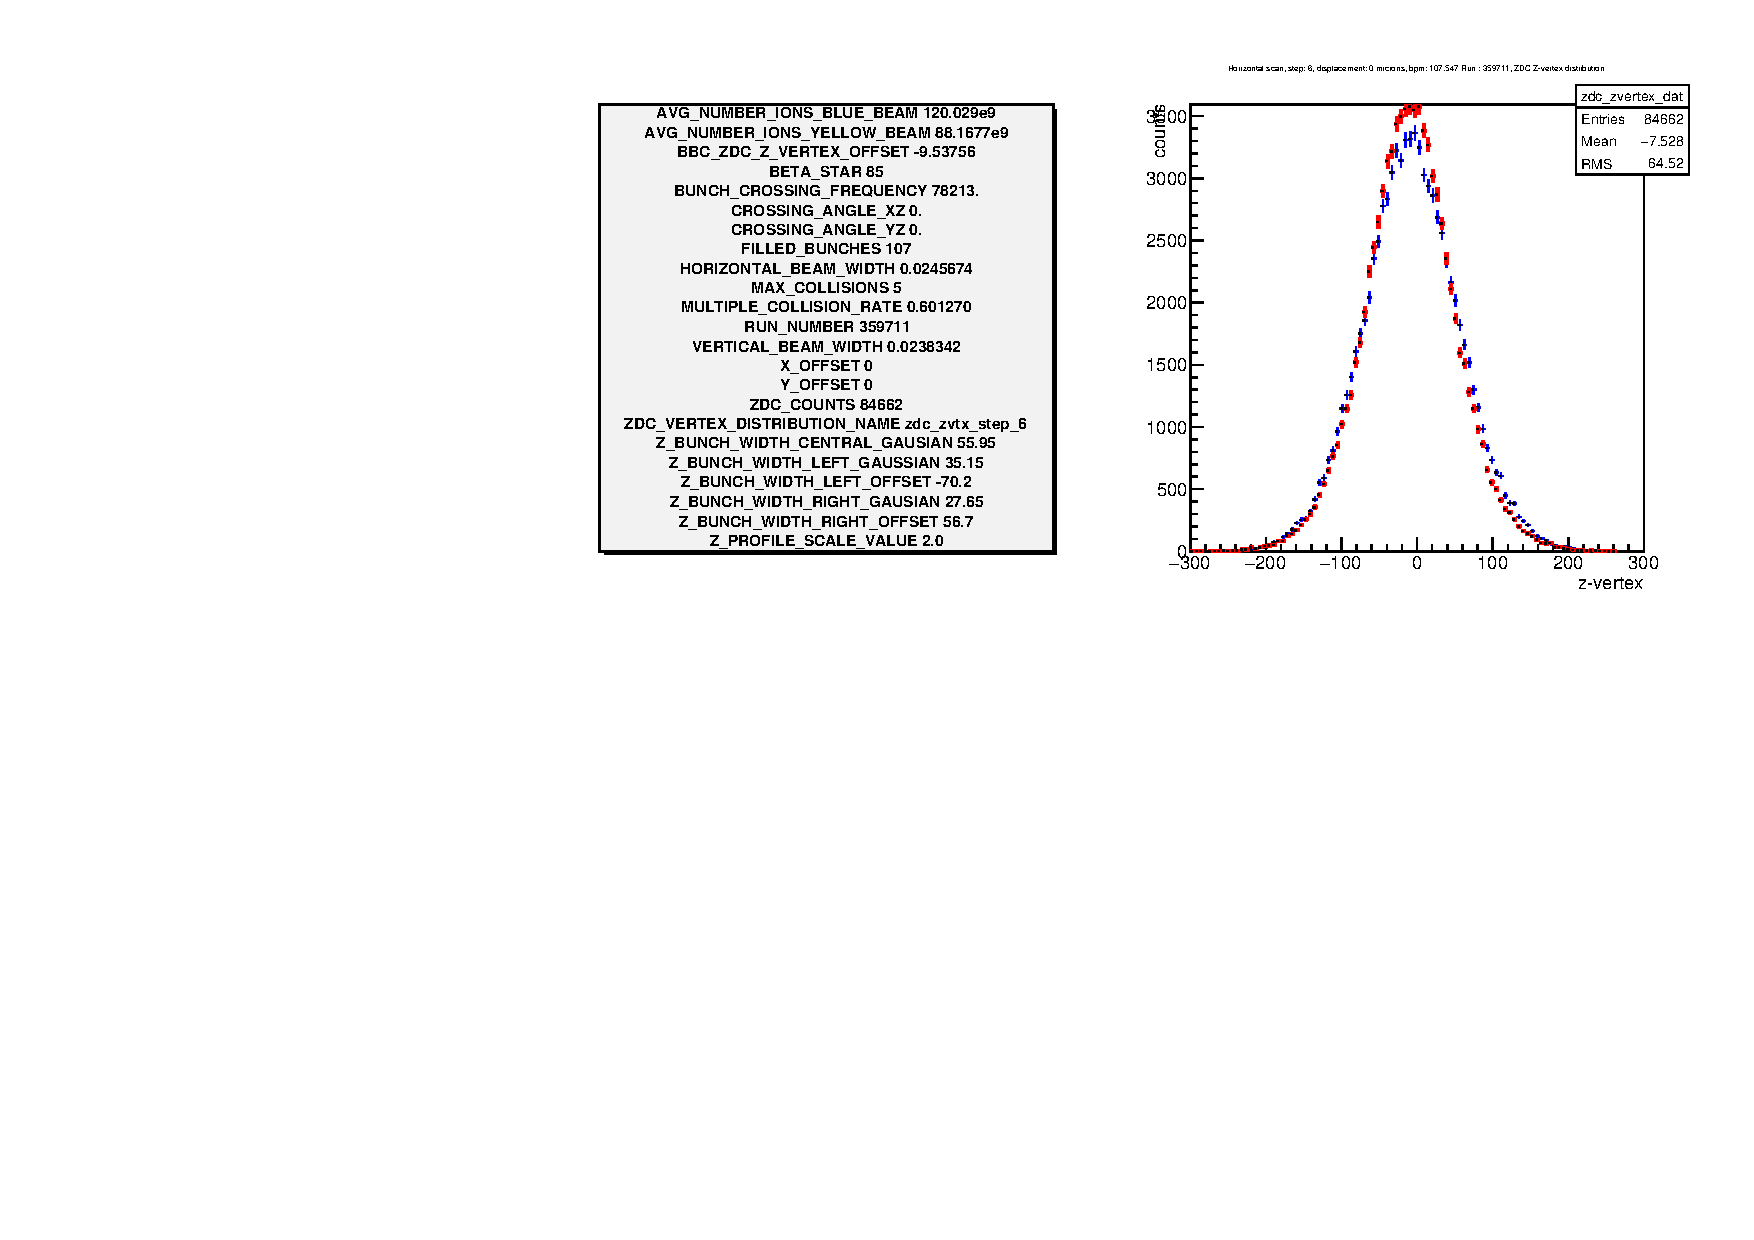
\includegraphics[width=\linewidth]{../OverlapTest/figs/359711_model1c_noangle_vertex.pdf}
\end{center}
\caption{Again, we have Amaresh's model, but have omitted the outer gausisan
contributions. If we set the crossing angle to zero, we get reasonable
convergence with the data.}
\label{fig:359711_model1c_noangle_vertex}
\end{figure}
\end{frame}

\begin{frame}
\frametitle{Amaresh Model, Central Gaussian Only, No Crossing Angle }
\begin{figure}
\begin{center}
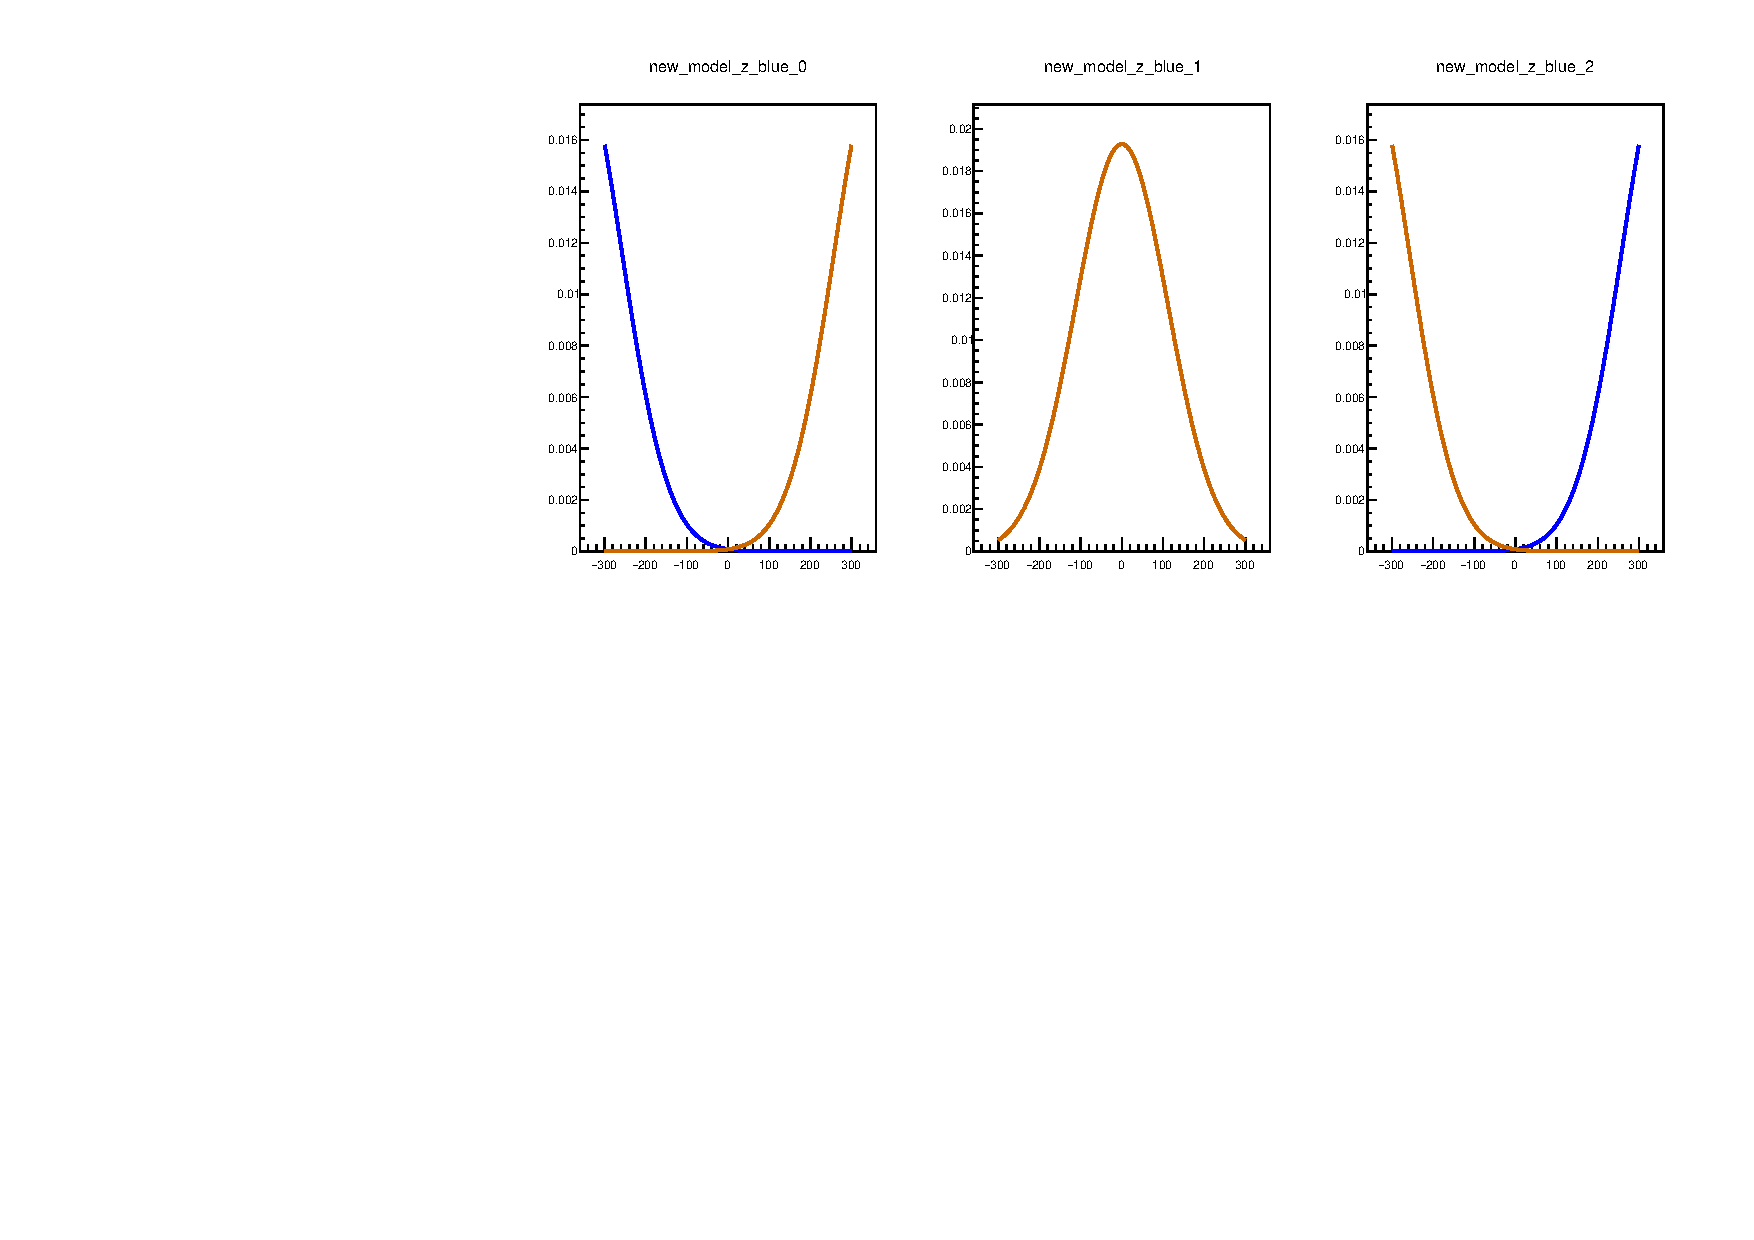
\includegraphics[width=\linewidth]{../OverlapTest/figs/359711_model1c_noangle_zprofile.pdf}
\end{center}
\caption{Snapshots of beam profiles as they collide, time increases from left to right }
\label{fig:359711_model1c_noangle_zprofile}
\end{figure}
\end{frame}

\subsection{Simple Gaussian Model - Width Based On Single Gaussian Fit to WCM Data }
\begin{frame}
\frametitle{Simple Single Gaussian, With Crossing Angle}
\begin{figure}
\begin{center}
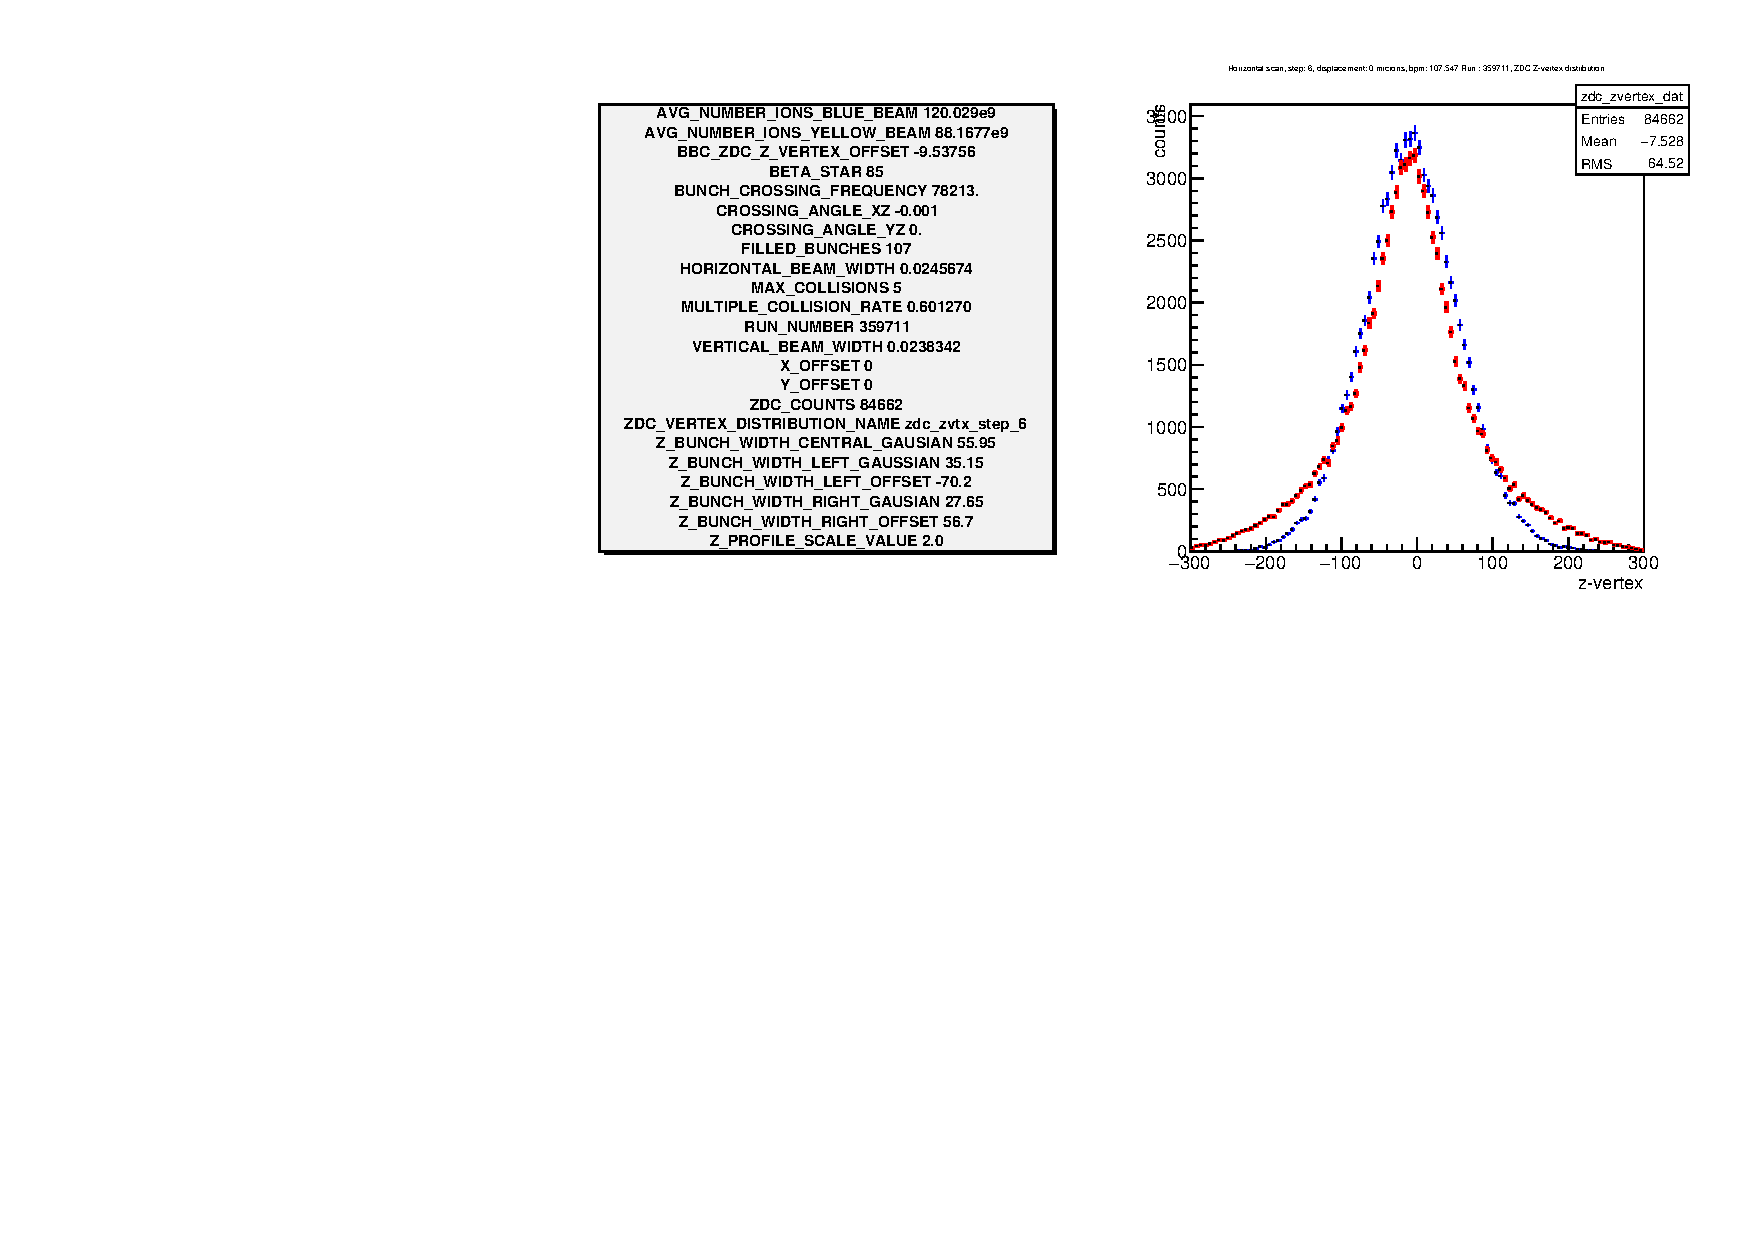
\includegraphics[width=\linewidth]{../OverlapTest/figs/359711_model3_angle_vertex.pdf}
\end{center}
\caption{Here, we ran the simulation again, but with a single gaussian whose
width is based on the overall width of the WCM distriubtion. This fit was done
separately from the WCM triple gaussian fit. }
\label{fig:359711_model3_angle_vertex}
\end{figure}
\end{frame}


\begin{frame}
\frametitle{Simple Single Gaussian, With Crossing Angle}
\begin{figure}
\begin{center}
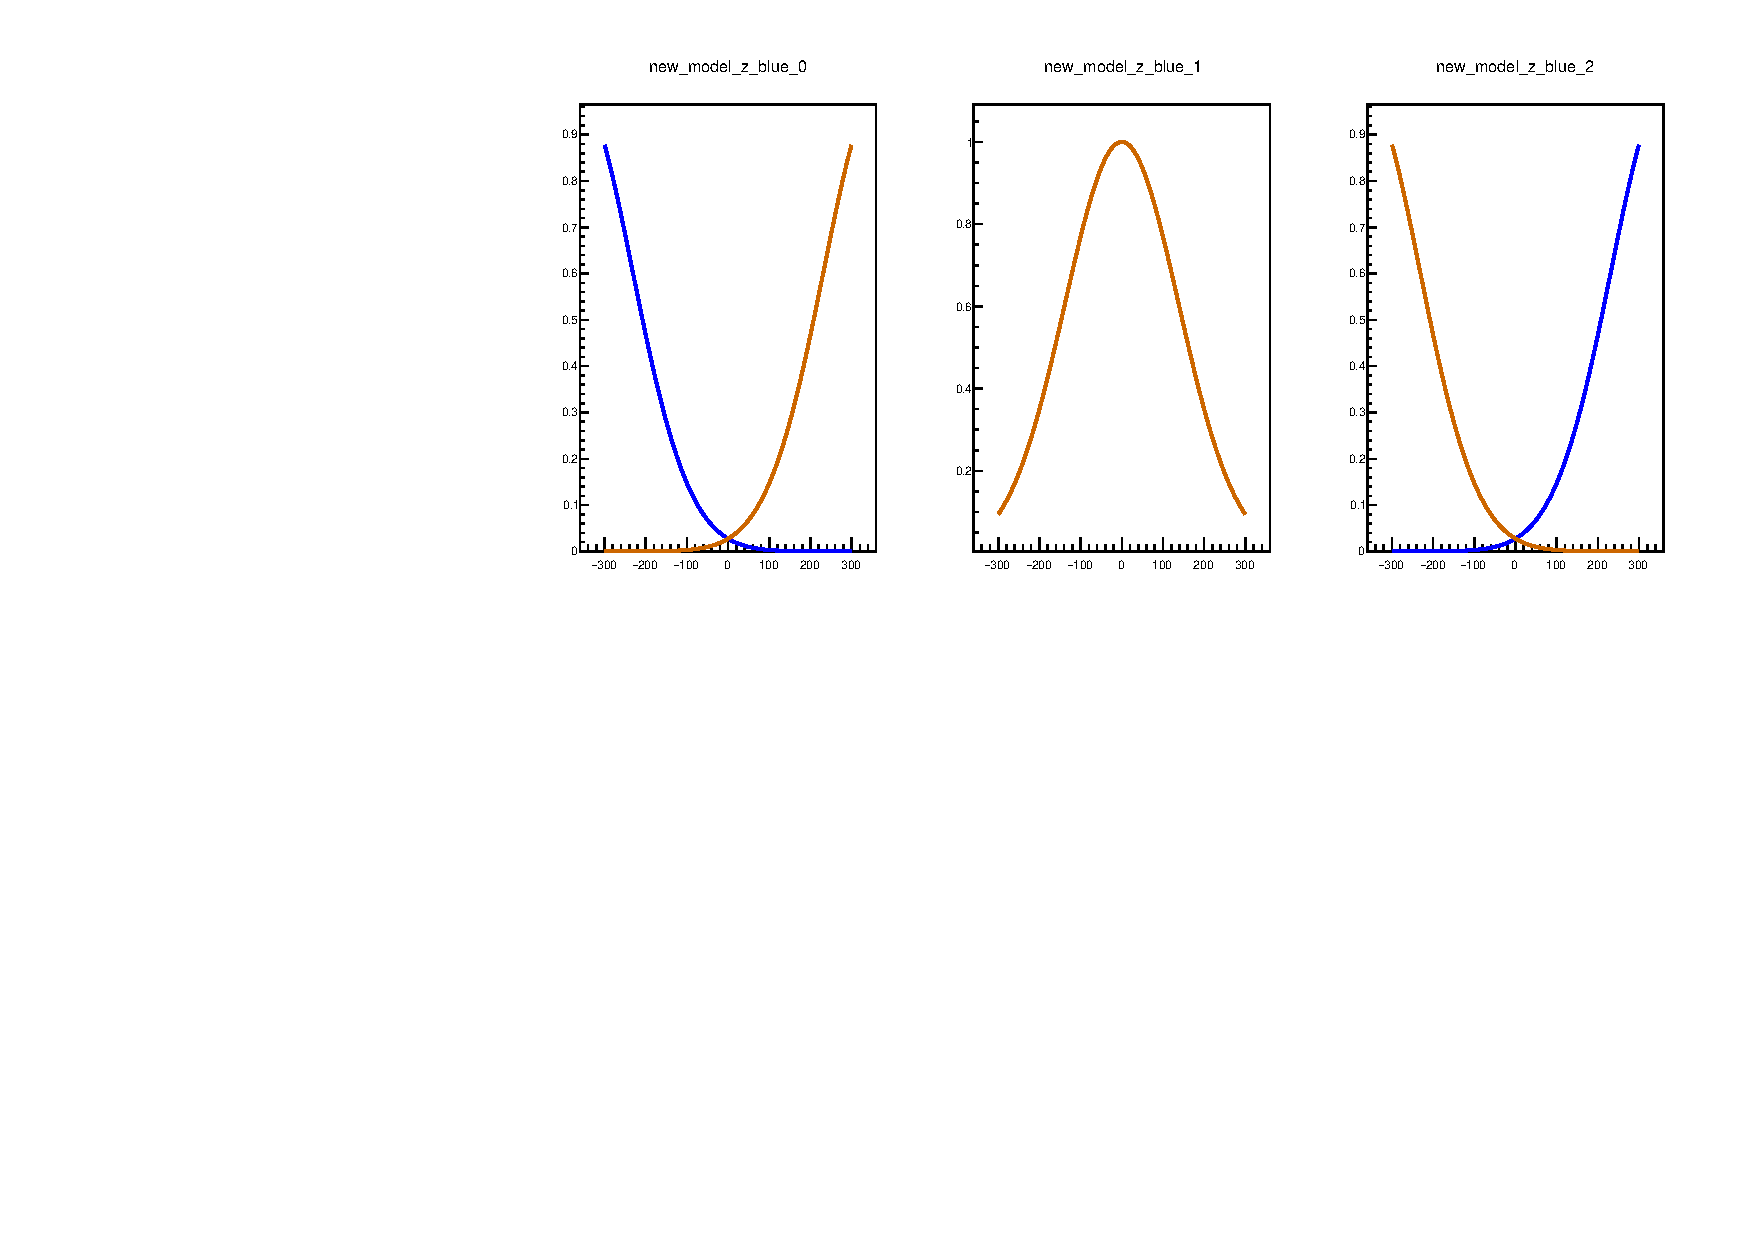
\includegraphics[width=\linewidth]{../OverlapTest/figs/359711_model3_angle_zprofile.pdf}
\end{center}
\caption{Snapshots of beam profiles as they collide, time increases from left to right }
\label{fig:359711_model3_angle_zprofile}
\end{figure}
\end{frame}


\begin{frame}
\frametitle{Simple Single Gaussian, No Crossing Angle}
\begin{figure}
\begin{center}
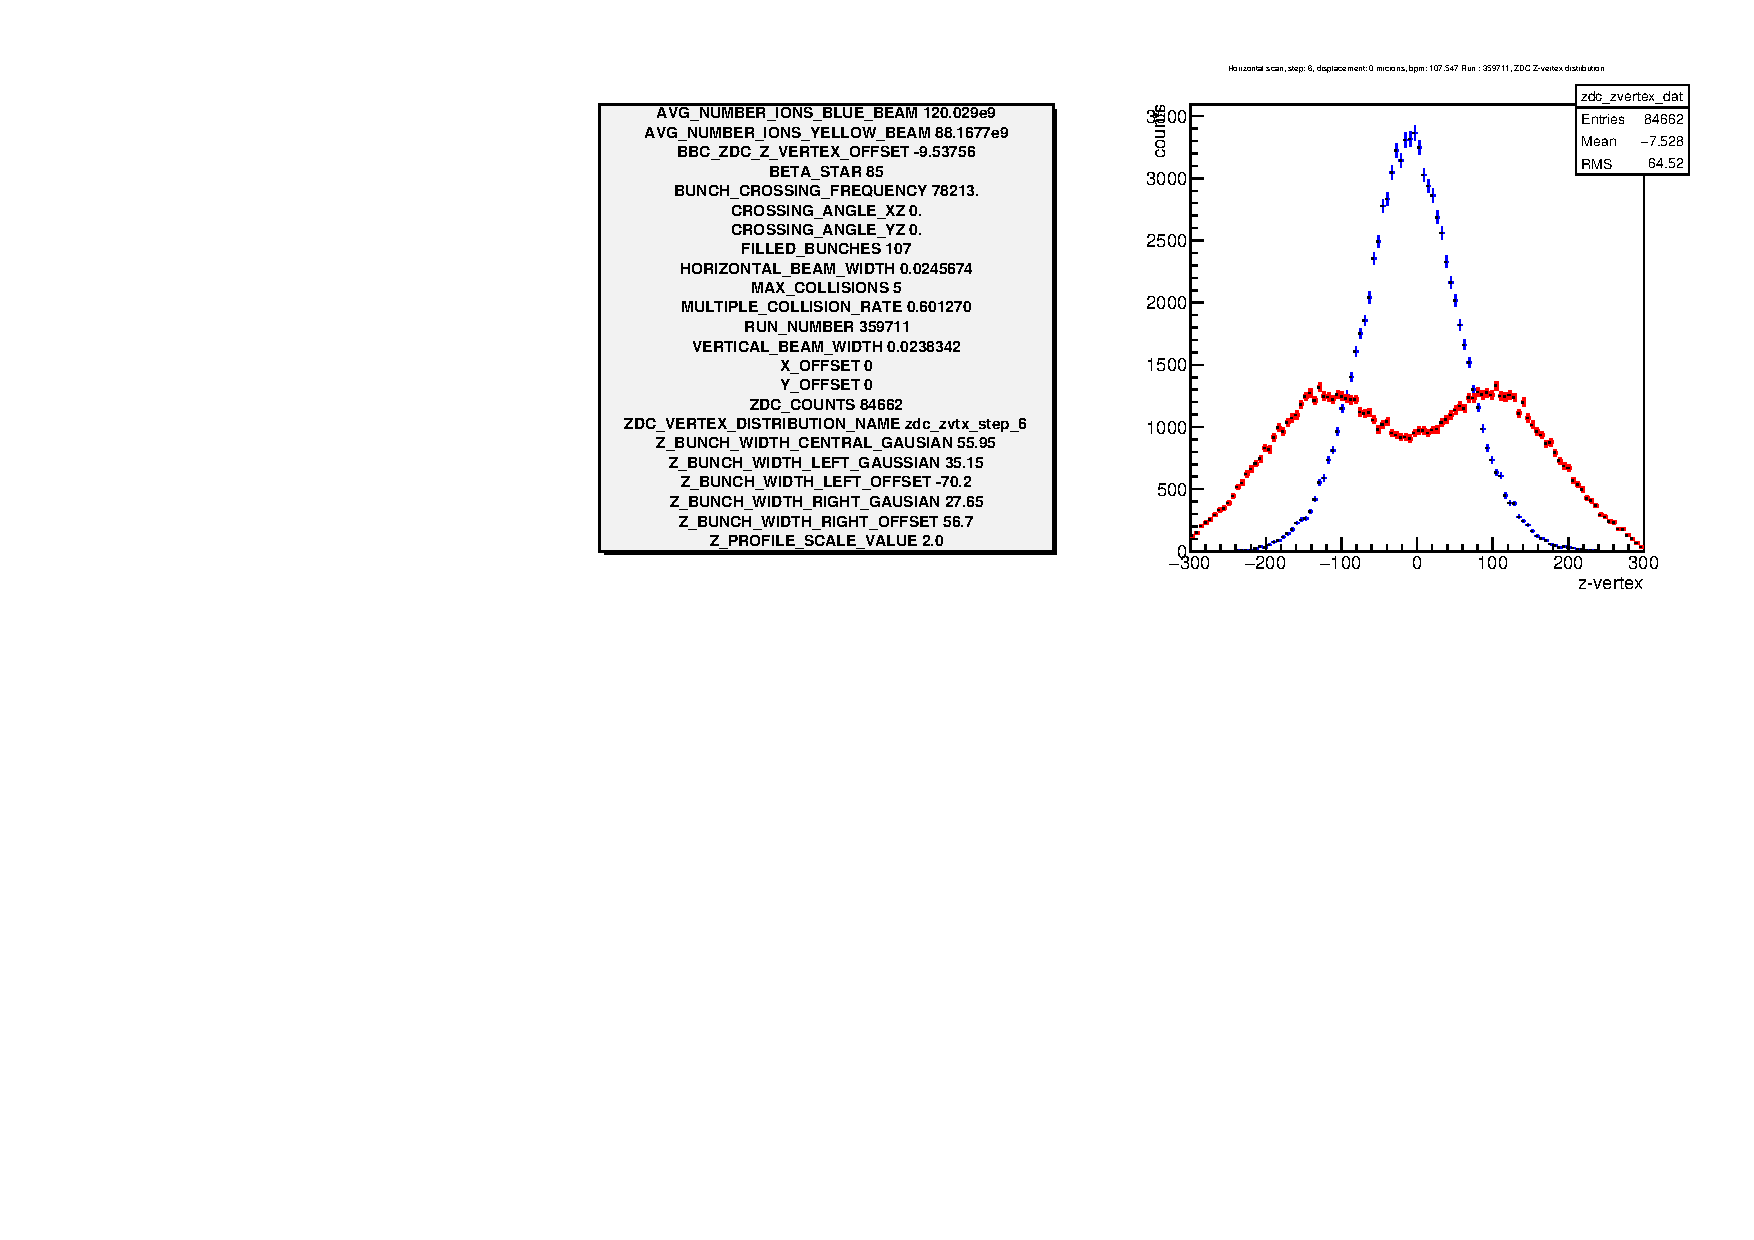
\includegraphics[width=\linewidth]{../OverlapTest/figs/359711_model3_noangle_vertex.pdf}
\end{center}
\caption{When we omit the crossing angle from the simulation, we again see the
humped structure re-appear. This directly contradicts our findings with the
central gaussian for Amaresh's model. However, Amaresh's width is 84 cm, while
this width is 138 cm}
\label{fig:359711_model3_noangle_vertex}
\end{figure}
\end{frame}


\begin{frame}
\frametitle{Simple Single Gaussian, No Crossing Angle}
\begin{figure}
\begin{center}
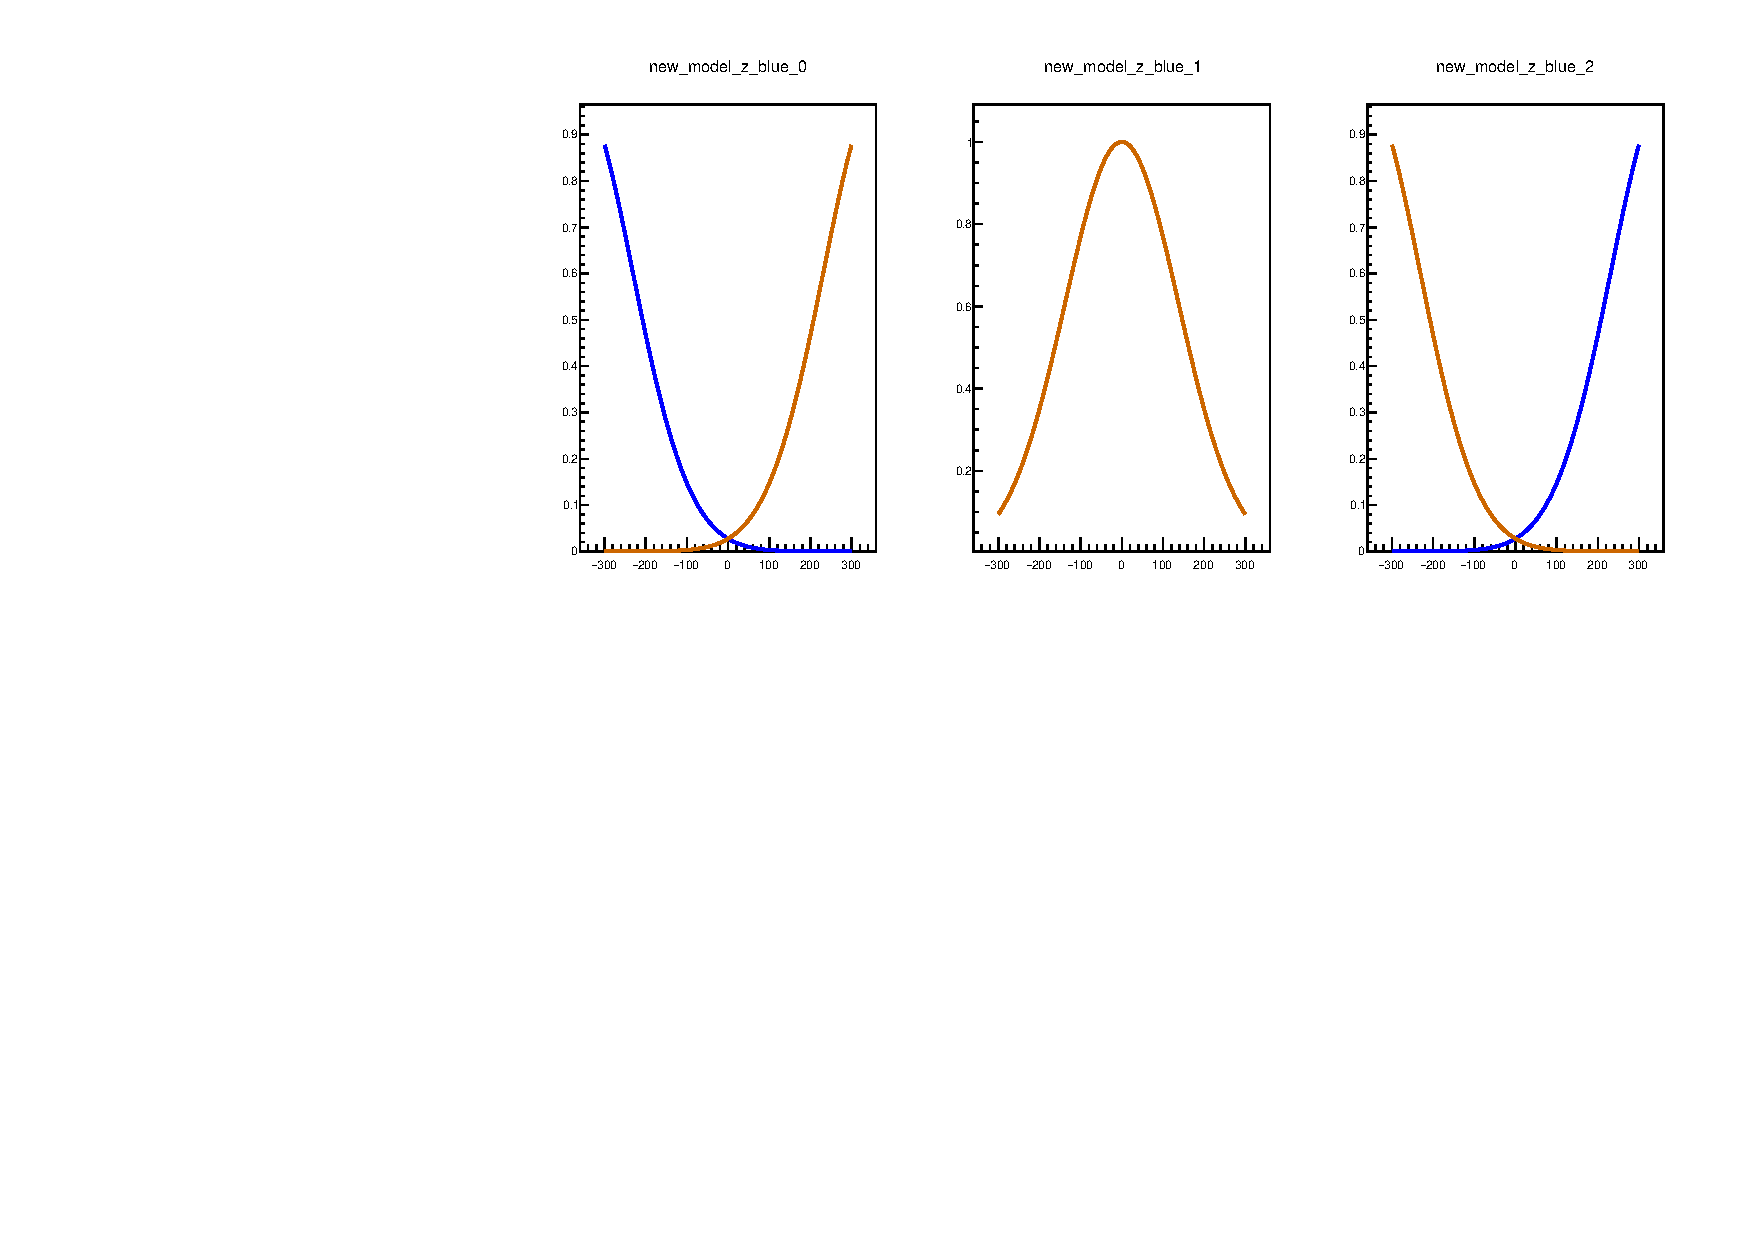
\includegraphics[width=\linewidth]{../OverlapTest/figs/359711_model3_noangle_zprofile.pdf}
\end{center}
\caption{Snapshots of beam profiles as they collide, time increases from left to right }
\label{fig:359711_model3_noangle_zprofile}
\end{figure}
\end{frame}


